\section{Theoretische und Technische Grundlagen}
% Farbe die angibt welchen Status der folgende Abschnitt hat:
% Eigentlicher Text:
In diesem Kapitel werden die technischen Grundlagen des Projektes, die zur Umsetzung nötig sind beschrieben.
\\Platzhalter kommt noch Text
\\Platzhalter kommt noch Text
\\Platzhalter kommt noch Text
\\Platzhalter kommt noch Text
\subsection{Robotik} % Manuel ca. 8
Die Robotik beschäftigt sich mit dem Entwurf, der Konstruktion sowie der Programmierung, Steuerung und dem Betrieb 
von Robotern.\footnote{\citep[vgl.][Definition Robotik]{Bendel.DefinitionRobotik}\label{note1}} Dabei umfasst die Robotik eine Vielzahl 
von Fachgebieten wie der Elektrotechnik, dem Maschienenbau, der Informatik sowie der Biologie und der Medizin.
\subsubsection{Roboter}
Was im Kontext der Robotik unter einem Roboter zu verstehen ist, ist gar nicht so einfach darzulegen, da es in Tat keine allgemein anerkannte Definition dieses Begriffs gibt, die seiner üblichen Verwendung entspricht.\footnote{\citep[vgl.][Mobile Roboter, Seite 2]{Hertzberg.MobileRoboter}\label{note2}}
\newline
Auch ohne eine vollkommen allgemeingültige und präzise Beschreibung eines Roboters zu sein, soll hier die \gls{vdi}-Richtline 2860 einen Eindruck darüber vermitteln, was in der Robotik mit Roboter gemeint ist. \newline
Die \gls{vdi}-Richtline 2860 von 1990 definiert einen Roboter wie folgt:\footref{note2}
\vspace{2mm}
\newline
\glqq{}\textit{Ein Roboter ist ein frei und wieder programmierbarer, multifunktionaler Manipulator mit mindestens drei unabhängigen Achsen, um Materialien, Teile, Werkzeuge oder spezielle Geräte auf programmierten,
variablen Bahnen zu bewegen zur Erfüllung der verschiedensten Aufgaben.}\grqq{}
\vspace{2mm}
\newline
Auch wenn diese Definition einige grundlegenden Eigenschaften eines Roboters darlegt, beschreibt diese den Begriff des Roboters im industriellen Kontext und trifft hauptsächlich auf stationäre Industrieroboter zu, wie sie in der Automobilfertigung beispielsweise als Schweiß- oder Lackierroboter verwendet werden. Die genannten programmierten Bahnen sind dort möglich, da die Arbeitsprozess und Umgebung auf den Roboter zugeschnitten und vollständig bekannt sind.\footref{note2} \newline
Im Gegensatz dazu, trifft dieser Aspekt auf mobile Roboter nicht zu, da sich diese meist in einer unbekannten, unstrukturierten und dynamischen Umgebung bewegen.
\subsubsection{Mobile Roboter}
Mobile Roboter bewegen sich selbständig durch eine sich meist ständig ändernde Umwelt. All ihre Aktionen sind somit von ihrer aktuellen Umgebung abhängen, die in ihrer konkrete Ausprägung erst zum Zeitpunkt der Aktionsausführung im Detail bekannt ist. 
\newline
Dieser grundsätzliche Unterschied zu stationären Robotern macht es unerlässlich das mobile Roboter ihre Umgebung ständig mittels Sensoren selbständig erfassen, die Sensordaten auswerten und auf Grundlage dessen ihre nächsten Aktionen planen.\footnote{\citep[vgl.][Mobile Roboter, Seite 2]{Hertzberg.MobileRoboter}\label{note3}}
\newline
Hinter dem Begriff des mobilen Roboters verbergen sich eine Vielzahl unterschiedlicher mobiler Systeme, welche
sich hinsichtlich ihrer Gestaltung, Arbeitsweise und ihrer Einsatzszenarien unterscheiden. Im Folgenden werden einige Beispiele für mobile Roboter dargelegt:
\begin{itemize}
	\item{\textbf{Shakey:}} Shakey ist ein mobiler Roboter der von 1966 bis 1972 an der am Stanford Research Institute entwickelt wurde. Seine Entwicklung leistete wichtige Beiträge für die Robotik sowie in der KI-Forschung im Bereich der Handlungsplanung und dem selbständigen Lernen.\footnote{\citep[vgl.][Mobile Roboter, Seite 5 f.]{Hertzberg.MobileRoboter}\label{note4}}
	%##################################################
	\item{\textbf{Spirit \& Opportunity:}} Spirit \& Opportunity sind zwei baugleiche Roboter die im Jahr 2003 von der NASA zum Mars geschickt wurden um den Himmelskörper zu erkunden. Die beiden Erkundungsroboter sind Radfahrzeuge mit flexiblem Fahrgestell, verfügen über eine Panoramakamera sowie Sensoren zur Untersuchung des Erdbodens und Gesteins. Obwohl die Roboter in Bezug auf ihrer grundsätzlichen Aktionen von der Erde aus ferngesteuert werden, ist eine autonome Steuerung, welche auf kurzfristige unerwartet Ereignisse, wie das Wegrutschen von Rädern reagiert aufgrund der langen Signallaufzeiten unverzichtbar. Die Roboter waren für eine
	Lebensdauer von 90 Marstagen ausgelegt, übertrafen diese aber bei weitem mit mehr als dem dreißig fachen.\footnote{\citep[vgl.][Mobile Roboter, Seite 8 f.]{Hertzberg.MobileRoboter}\label{note4}}
	%##################################################
	\item{\textbf{Stanley:}} Stanley ist ein vollständig autonomer Roboter der 2005 am Grand Challenge Wetbewerb teilnahm und diesen gewann. Bei diesem Wettbewerb mussten Fahrzeuge ohne Eingriff von Menschen eine festgelegte, jedoch nicht markierte Strecke von rund 213 km von einem definierten Start- zu einem definierten Zielpunkt zurücklegen. Die Strecke führte durch die Mojave-Wüste in den USA. Bei Stanley handelt es sich um einen modifizierter VW Touareg, dem Sensoren zur Umgebungswahrnehmung und Bordrechner zur Bearbeitung des Kontrollprogramms eingebaut wurden. Stanleys wichtigste Umgebungssensoren waren mehrere Laserscanner und eine Kamera. Stanley meisterte die 213 km lange Strecke welche unter anderem durch felsige oder sandige Bereiche sowie durch Wasserläufe führte in knapp unter 7 Stunden.\footnote{\citep[vgl.][Mobile Roboter, Seite 9 f.]{Hertzberg.MobileRoboter}\label{note5}}
	%##################################################
\end{itemize}
Allein diese drei Beispiele zeigen wie sehr sich mobile Roboter im Aufbau, Einsatzort und Aufgabe unterscheiden. Neben reinen Forschungs- sowie wissenschaftlich-technischen Gründen Mobile Roboter zu bauen, sind diese auch aus wirtschaftlicher Perspektive interessant und haben gerade in den letzten Jahren an Marktpotenzial gewonnen.
\newline
Zu den Vertretern mobiler Roboter im kommerziellen Bereich zählen zum Beispiel Service-Roboter, Erkundungsroboter und Bergungsroboter, Humanoide Roboter sowie Haushaltsroboter.
\subsubsection{Sensorik}
Um mit der Umgebung interagieren zu können, müssen mobile Roboter diese wahrnehmen, dazu dienen Sensoren. Diese ermöglichen es dem Roboter Informationen über seine Umwelt und über seinen Zustand zu sammeln um darauf Aufbauen seine nächsten Interaktionsschritte zu planen.
\paragraph{Klassifizierung}
Sensoren lassen sich anhand zweier Aspekten klassifizieren, zum einen hinsichtlich des Objektes über welches sie Informationen liefern (die Umwelt oder den Roboter selbst) und anderseits hinsichtlich ihrer Arbeitsweise.\footnote{\citep[vgl.][Mobile Roboter, Seite 24]{Hertzberg.MobileRoboter}\label{note6}}
\begin{itemize}
	\item{\textbf{Propriozeptive Sensoren}} -- Diese Art der Sensoren bestimmen eine Messgröße des Roboters selbst und haben keine \glqq{}Kontakt\grqq{} zur Umwelt z.B Bestimmung der Lage Aufgrund eines Neigungssensors.
	\item{\textbf{Exterozeptive Sensoren}} -- Im Gegensatz zu den propriozeptive Sensoren gewinnen diese Sensoren Informationen aus Messgrößen der Umwelt beispielsweise die Bestimmung der Orientierung in Bezug auf die Umwelt.
	\item{\textbf{Aktive Sensoren}} -- Aktive Sensoren senden aktive Energie in ihre Umwelt aus und Erfassen anschließend die zurückkehrenden Signale wie dies beispielsweise ein Ultraschallsensor tut.
	\item{\textbf{Passive Sensoren}} -- Diese Sensoren senden nicht aktiv aus sondern erfassen ausschließlich die von der Natur aus vorhandenen Signale wie z.B. das einfallende Licht durch eine Kamera.
\end{itemize}
Die folgenden Tabelle zeigt beispielhaft die Einordnung einiger Sensoren:
\begin{table}[ht]
	\begin{tabular}{|p{4,5cm}|p{4,0cm}|p{4,0cm}|} \hline
		     	                & Aktive Sensoren      & Passive Sensoren   \\ \hline
		Propriozeptive Sensoren & 
			-- & 
			Inkrementalgeber, \newline Neigungssensor, \newline Gyroskop   \\ \hline
		Exterozeptive Sensoren  & 
			Ultraschallsensor,  \newline Laserscanner, \newline Infrarotsensor, \newline Radar    & 
			Kontaktsensor, \newline Kompass, \newline Kamera, \newline GPS      \\ \hline 
	\end{tabular}
	\centering
	\caption[Einordnung von Sensoren]{Einordnung von Sensoren}
\end{table}
\paragraph{Eigenschaften}
Neben der Arbeitsweise gibt es noch weitere Eigenschaften die maßgeblich beeinflussen wann, wie und für welchen Zweck ein jeweiliger Sensor eingesetzt wird. Zu den wichtigsten Eigenschaften zählen:\footnote{\citep[vgl.][Mobile Roboter, Seite 26 f.]{Hertzberg.MobileRoboter}\label{note7}}
\begin{itemize}
	\item{\textbf{Messbereich}} -- Jeder Sensor hat einen bestimmten Bereich, in dem die gemessenen Daten valide sind d.h. der Bereich in dem die Messabweichungen innerhalb der festgelegten Grenzen bleibt.
	\item{\textbf{Dynamik}} -- Die Dynamik beschreibt das Verhältnis von Ober- zu Untergrenze des Messwerts.
	\item{\textbf{Auflösung}} -- Die Auflösung beschreibt wie granular eine physikalische Größe ermittelt werden kann d.h sie gibt den kleinsten messbaren Unterschied zweier Messwerte an.
	\item{\textbf{Linearität}} -- Unter der Linearität eines Sensors versteht man die Abhängigkeit des Messwerts von der tatsächlichen Größe.
	\item{\textbf{Messfrequenz}} -- Die Messfrequenz gibt an wie viele einzelne Messungen innerhalb eines bestimmten Zeitraums der Sensor liefert.
\end{itemize}
Da jegliche Messung fehlerbehaftet ist, weisen auch die von Sensoren ermittelte Messwerte gewisse Fehler auf.\footnote{\citep[vgl.][Mobile Roboter, Seite 27]{Hertzberg.MobileRoboter}\label{note8}}
\newline
Damit die Robotersteuerung darauf Rücksicht nehmen kann müssen die entsprechenden Kenngrößen der Sensoren bekannt sein. Folgende Größen sind mit Bezug auf Sensorfehler von Bedeutung:\footnote{\citep[vgl.][Mobile Roboter, Seite 27 f.]{Hertzberg.MobileRoboter}\label{note9}}
\begin{itemize}
	\item{\textbf{Empfindlichkeit}} -- Wie groß eine Wertänderung der Ausgangsgröße sein muss damit dies der Sensor registriert, wird als Empfindlichkeit bezeichnet. Eine hohe Empfindlichkeit hat oft eine hohe Störanfälligkeit zur Folge.
	\item{\textbf{Messfehler}} -- Als Messfehler oder absoluten Fehler bezeichnet man die Differenz des gemessenen Wertes m und des tatsächlichen Wertes.
	\item{\textbf{Genauigkeit}} -- Die Genauigkeit oder der relative Fehler ist der prozentuale	Wert einer Abweichung in Bezug zum tatsächlichen Wert.
\end{itemize}
\paragraph{Kenngrößen}
In der Robotik finden zahlreiche Sensoren Anwendung, um es einem mobilen Systems zu ermöglichen verschiedene Kenngrößen zu ermitteln. Im Folgenden werden einiger dieser und die dazu geeigneten Sensoren vorgestellt.
\begin{itemize}
	\item{\textbf{Bewegungsmessung}} -- Eine Möglichkeit der Bewegungsmessung ist die Drehwinkelmessung. Diese ermöglicht die Erfassung der Drehungen von Rädern oder anderen rotierenden Elementen eines mobilen Roboters. Dies ermöglicht es mittels Odometire die Geschwindigkeit und Orientierung eines mobilen Roboters zu bestimmen, siehe Abschnitt \eqref{odometrie}. Zur Drehwinkelmessung dienen Impuls- sowie Inkrementalgeber welche mechanisch, photo-elektrisch und elektro-magnetisch arbeiten.\footnote{\citep[vgl.][Mobile Roboter, Seite 28 ff.]{Hertzberg.MobileRoboter}\label{note10}}
	\newline
	Eine weitere Möglichkeit der Bewegungsmessung ist die Beschleunigungsmessung. Dabei werden Bewegungen über die Massenträgheit bei Beschleunigungen gemessen und über die Zeit integriert, weshalb man auch von Trägheitsmessung spricht.\footnote{\citep[vgl.][Mobile Roboter, Seite 31]{Hertzberg.MobileRoboter}\label{note11}} Dazu werden heute meist
	piezo-elektronische Gyroskope verwendet welche Dreh- und Linearbeschleunigungen bezüglich aller drei Raumachsen erfassen.\footnote{\citep[vgl.][Mobile Roboter, Seite 32 ff.]{Hertzberg.MobileRoboter}\label{note11}}
	%############################################################
	\item{\textbf{Ausrichtungsmessung}} -- Neben der Bestimmung der geografische Position eines Roboters mittels Beschleunigung- und Drehratensensoren ist auch dessen Ausrichtung bzw. Lage im Raum eine wichtige Größe. Zur Bestimmung der Ausrichtung werden Kompasse sowie Inklinometer verwendet, welche den Neigungswinkel zur Erdanziehungsrichtung bestimmen.\footnote{\citep[vgl.][Mobile Roboter, Seite 32 f.]{Hertzberg.MobileRoboter}\label{note12}}
	%############################################################
	\item{\textbf{Entfernungsmessung}} -- Die Entfernungsmessung dient der Bestimmung des Abstands zu Objekten z.B. zur Kollisionsvermeidung. 
	\newline
	Es gibt verschiedene Arten von Sensoren zur Entfernungsmessung viele basieren auf dem Prinzip der Laufzeitmessung, wie Ultraschallsensoren oder Laserentfernungsmesser. Darüber hinaus gibt es auch Sensoren, die mittels Triangulation (Inrarotsensor) oder dem Verhältnis zwischen ausgesandter und zurückkehrender Energie (Radar) die Entfernung zu Objekten bestimmen.\footnote{\citep[vgl.][Mobile Roboter, Seite 36 f.]{Hertzberg.MobileRoboter}\label{note13}}
\end{itemize}
Neben diesen elementaren Kenngrößen gibt es zahlreiche weitere die für ein entsprechendes mobile System von Bedeutung sind. Dies ist beispielsweise eine globale Positionsbestimmung mittels \gls{gps} oder die Dedektion von Objekten und geografischen Strukturen durch Kameras oder 2D-/3D-Laserscanner.
\subsubsection{Sensordatenverarbeitung \& Steuerung}
Generell unterscheidet man zwischen zwei grundlegenden Arten der Steuerung, einer offenen und geschlossenen. Das typische Kontrollprogramm eines Roboters in der Automatisierung läuft in einer offenen Steuerung d.h. es werden keine Sensordaten aus der Umgebung erfasst bzw. berücksichtigt. Dies ist dort möglich, da sich dort Roboter auf vordefinierten Bahnen und in eine auf sie zugeschnittenen Umgebung bewegen.
\newline
Prozesssteuerungen dieser Art haben ihre Grenzen da, wo sich ein Roboter in einer unstrukturierten Umgebung bewegt und von Ereignissen oder Parametern abhängt, die nicht kontrollierbar bzw. vorab nicht bekannt sind.\footnote{\citep[vgl.][Mobile Roboter, Seite 3 f.]{Hertzberg.MobileRoboter}\label{note14}}
Mobile Roboter verfügen über eine geschlossene Steuerung bei der eine Rückkopplung der Umgebung durch Sensordaten erfolgt. In einem iterativen Verfahren werden die von den Sensoren ermittelten Umgebungsdaten bei der Planung von Steuerbefehle einbezogen, die resultierenden Aktionen ausgeführt was ggf. die Umgebung verändert, woraufhin der Regelkreis erneut beginnt.
\begin{figure}[ht]
	\centering
		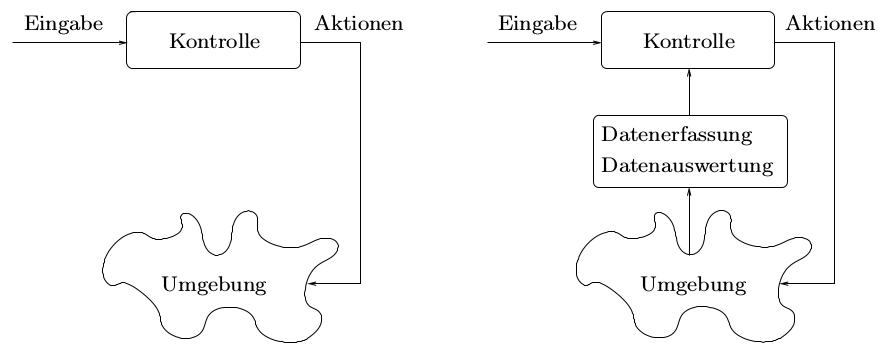
\includegraphics[width=0.90\textwidth]{images/technische_grundlagen/Steuerungsarten.png}
		\caption[Vergleich Offene und Geschlossene Steuerung]{Links: Offene Steuerung. Rechts: Geschlossene Regelung mit Rückkopplung}
		\cite{Hertzberg.MobileRoboter}
\end{figure}
\newline
Die Sensordatenverarbeitung hat die Aufgabe, die durch die Sensoren erfassten Daten zu verarbeiten, aufzubereiten und sie für komplexere Anwendungen nutzbar zu machen. Dazu gehören die Filterung der Daten, Extraktion bestimmter Merkmale sowie weiterführende Berechnung von Kenngrößen und Informationen.\footnote{\citep[vgl.][Mobile Roboter, Seite 67]{Hertzberg.MobileRoboter}\label{note15}}
\paragraph{Odometrie \& Koppelnavigation}\label{odometrie}
Die Odometrie bezeichnet eine Methode zur Berechnung von Position und Orientierung eines mobilen Systems anhand von Bewegungsdaten. Räder basierte Systeme benutzen dafür die Anzahl der Radumdrehungen, während laufende Systeme die Anzahl ihrer Schritte verwenden. Ist beispielsweise der Raddurchmesser bekannt, so kann über die Anzahl $n$ der Radumdrehungen (welche z.B. mittels Inkrementalgebern erfasst wird) zwischen zwei Messzeitpunkten und dem Radumfang $\pi \cdot d$, wobei $d$ den Raddurchmesser darstellt, die zurückgelegte Wegstrecke $\Delta{}s$ berechnet werden:
\begin{equation}
\Delta{}s = \pi \cdot d \cdot n
\end{equation}
Unter Koppelnavigation versteht man die Bestimmung der Position eines mobilen Systems relativ zu einem Referenzpunkt (Startposition) entweder durch die inkrementelle Integration der zurückgelegten Wegstrecken unter Berücksichtigung der Orientierung (Winkeländerung) oder der Geschwindigkeit des Systems unter Berücksichtigung der Winkelgeschwindigkeit.\footnote{\citep[vgl.][Mobile Robotik, Seite 98]{Nehmzow.MobileRobotik}\label{note16}}
\newline
Ist der Ausgangspunkt eines Roboters, die zurückgelegte Strecke bzw. Geschwindigkeit sowie die Fahrtrichtung genau bekannt, kann die Navigationskomponente die Bewegung des Roboterssystms über die Zeit integrieren und so die aktuelle Position und Orientierung des Roboters bestimmen.\footnote{\citep[vgl.][Handbuch Robotik, Seite 107 f.]{Haun.HandbuchRobotik}\label{note17}}
\newline
Im eindimensionalen Fall (keine Richtungsänderungen) ergibt sich aus dem Startpunkt $s_{alt}$ und  der zurückgelegten Wegstrecke $\Delta{}s$ aus Gleichung (1), für die aktuelle Position $s_{neu}$ die Gleichung:
\begin{equation}
s_{neu} = s_{alt} + \Delta{}s
\end{equation}
Für eine zweidimensionale Bewegung in einem 2-dimensionalen kartesische Bezugssystem in dem sich die Position eines Roboters als Koordinate durch x- und y-Punkt darstellen lässt ergibt sich die
Position $(x_{n},y_{n})$ und die Orientierung $\theta{}_{n}$ zum Iterationsschritt (Messpunkt) $n$ durch die Formeln:
\begin{equation}
x_{n} = x_{0} + \sum_{i=1}^{n} \Delta{}s_{i} \cdot cos(\theta{}_{i})
\end{equation}
\begin{equation}
y_{n} = y_{0} + \sum_{i=1}^{n} \Delta{}s_{i} \cdot sin(\theta{}_{i})
\end{equation}
\begin{equation}
\theta{}_{n} = \theta{}_{0} + \sum_{i=1}^{n} \Delta{}\theta{}_{i}
\end{equation}
Wobei $(x_{0},y_{0})$ der Startpunkt und $\theta{}_{0}$ die Startorientierung sowie $\Delta{}s_{i}$ die zurückgelegte Wegstrecke und $\Delta{}\theta{}_{i}$ die Richtungsänderung innerhalb eines Iterationsschritt darstellt.
\newline
Die Odometrie ist im Zusammenspiel mit der Koppelnavigation ein grundlegendes Navigationsverfahren für bodengebundene Fahrzeuge aller Art. Allerdings besteht ein wesentliches Problem darin, dass ein Robotersystem seine Bewegungen absolut präzise messen können muss, damit die Odometrie bzw. Koppelnavigation richtige Werte liefert. Dies ist unter Umständen aufgrund
von Problemen wie beispielsweise variierender Raddurchmesser dem Durchdrehen oder Gleiten der Räder erschwert wird.\footnote{\citep[vgl.][Handbuch Robotik, Seite 108]{Haun.HandbuchRobotik}\label{note18}}
\newline
Wegen diesen Problemen finden sich kaum Roboternavigationssysteme, welche ausschließlich eine Koppelnavigation zur Bestimmung von Position und Orientierung verwenden. Es gibt zwar Navigationssysteme, welche die Koppelnavigation verwenden, jedoch beziehen diese noch weitere Sensorinformationen, wie beispielsweise Beschleunigungswerte zur Bestimmung der Position und Ausrichtung mit ein.\footnote{\citep[vgl.][Mobile Robotik, Seite 115]{Nehmzow.MobileRobotik}\label{note19}}
\subsubsection{Antriebsarten}
Die entscheidende Eigenschaft des mobilen Roboters ist die Fähigkeit sich selbständig durch seine Umwelt zu bewegen. Um dies zu realisieren gibt es eine Vielzahl unterschiedlichster Fortbewegungsarten, beispielsweise in Form von schreitenden, kriechenden oder krabbelnden, sowie fliegenden, schwimmenden oder tauchenden Robotern.\footnote{\citep[vgl.][Mobile Roboter, Seite 103]{Hertzberg.MobileRoboter}\label{note20}}
\newline
Um den Umfang dieser Ausarbeitung überschaubar zu halten, beschränken wir uns auf die Darstellung von radgetriebenen Robotern.
\medskip
\newline
Hinsichtlich Rad- und Achsenanzahl, Anordnung der Räder sowie dem Verhältnis zwischen angetrieben und freilaufenden, als auch lenkbaren zu unlenkbaren Rädern gibt es eine Vielzahl von Möglichkeiten den Antrieb von mobilen Robotern zu konzipieren. Die folgende Abschnitte geben einen Überblick über die gängigsten radbasierten Antriebskonzepte.\footnote{\citep[vgl.][Mobile Roboter, Seite 107 f.]{Hertzberg.MobileRoboter}\label{note21}}
\begin{wrapfigure}{r}{0.30\textwidth}
	\vspace{+0.5cm}
	\begin{center}
		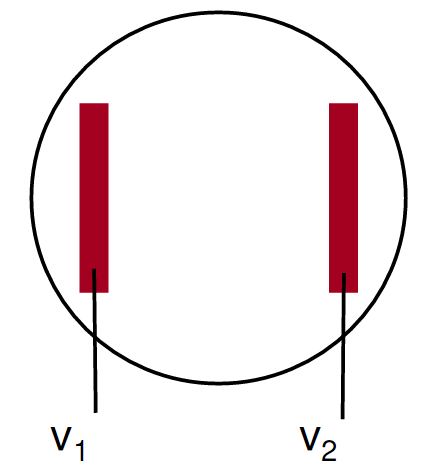
\includegraphics[width=0.25\textwidth]{images/technische_grundlagen/Differentialantrieb.png}
	\end{center}
	\caption{Einachsige Lenkung}
	\label{fig:einachsenlenkung}
\end{wrapfigure}
\paragraph{Differentialantrieb}
Dieser Antrieb besteht aus zwei voneinander unabhängig angetriebene, starren Rädern die sich auf einer Achse befinden. Zusätzlich gibt es meist ein oder auch mehrere passiv mitlaufenden Stützrädern, die sich frei drehen können. Je nachdem, wie und in welchem Verhältnis zueinander die beiden Antriebsräder sich drehen, fährt der Roboter gerade aus, eine mehr oder weniger weite Rechts- oder Linkskurve oder dreht sich auf der Stelle.\\
Vorteile dieses Antriebs sind seine einfache Mechanik und gute Manövierbarkeit, welcher jedoch eine Radregelung des Antriebs in Echtzeit erfordert.
\begin{wrapfigure}{r}{0.30\textwidth}
	\vspace{-0.25cm}
	\begin{center}
		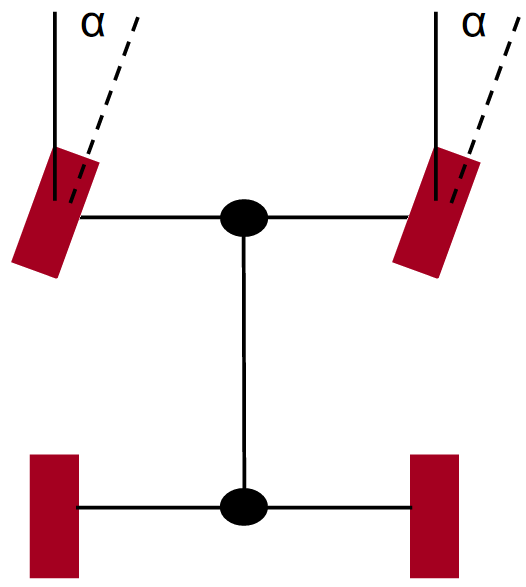
\includegraphics[width=0.20\textwidth]{images/technische_grundlagen/Einachsenlenkung.png}
	\end{center}
	\caption{Einachsige Lenkung}
	\label{fig:einachsenlenkung}
\end{wrapfigure}
\paragraph{Einachsige Lenkung}
Dieses Antriebsprinzip entspricht dem aus gängigen PKWs bekannten Konzept. Von den vier Rädern, von denen jeweils zwei an einer Achse angebracht sind, sind beide Räder einer Achse lenkbar. Für den Antrieb ist es möglich eine der beide Achsen, als auch beide anzutreiben. 
\newline
Der Vorteil dieses Antriebskonzeptes ist die gute Stabilität und die Möglichkeit der Trennung von Antrieb und Lenkung jedoch ist die Nanövierbarkeit eingeschränkter als bei den anderen Antriebsarten.
\begin{wrapfigure}{r}{0.30\textwidth}
	\vspace{+0.25cm}
	\begin{center}
		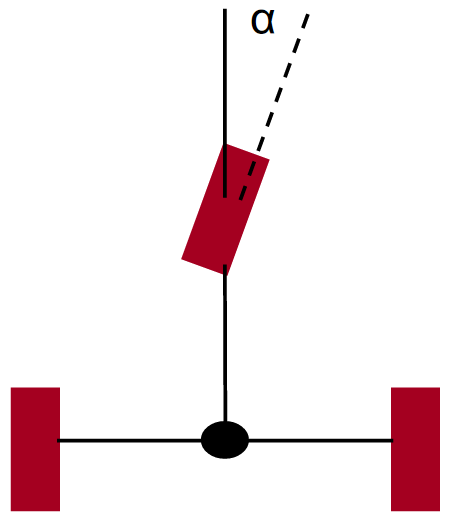
\includegraphics[width=0.20\textwidth]{images/technische_grundlagen/Dreiradantrieb.png}
	\end{center}
	\caption{Dreirad-Antrieb}
	\label{fig:einachsenlenkung}
\end{wrapfigure}
\paragraph{Dreirad-Antrieb}
Bei diesem Antriebskonzept verfügt der mobile Roboter über zwei freilaufenden Räder auf einer Achse sowie einem einzelnen angetriebenen und gelenkten Rad, welches zentral vor den beiden anderen Rädern angebracht ist. Es ist auch möglich, dass ein Motor beide Hinterräder antreibt, und das Vorderrad allein der Lenkung dient.
\newline
Die einfache Mechanik dieser Antriebsform ist ein Vorteil, jedoch ist die Manövierbarkeit eingeschränkter als beim Synchro- oder Differentialantrieb und die Stabilität ist geringer, als bei der Einachsen Lenkung, die über ein zusätzliches Rad an der Vorderachse verfügt.
\begin{wrapfigure}{r}{0.30\textwidth}
	\vspace{-0.8cm}
	\begin{center}
		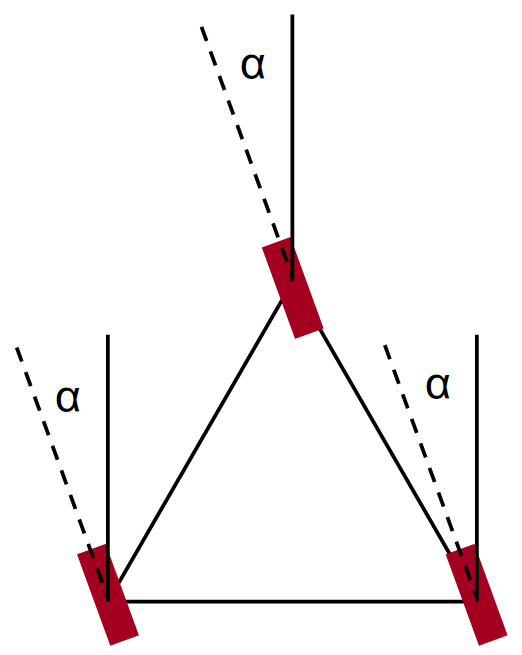
\includegraphics[width=0.25\textwidth]{images/technische_grundlagen/Synchroantrieb.png}
	\end{center}
	\caption{Einachsige Lenkung}
	\label{fig:einachsenlenkung}
\end{wrapfigure}
\paragraph{Synchro-Antrieb}
Der Synchro-Antrieb hat die selbe Radanordnung, wie der Dreirad-Antrieb, jedoch werden die drei Räder synchron angetriebene und sind auch nur synchron drehbar. Die Räder haben somit immer die selbe Ausrichtung und drehen sich auch mit der selben Geschwindigkeit. Eine Drehung des Roboters bzw. der auf dem Antrieb angebrachte Plattform ist nicht direkt möglich.
\newline
Durch die synchrone Lenkung und den synchronen Antrieb der Räder erfordert diese Antriebsform eine weitaus komplexere Mechanik, als die anderen Antriebsarten, garantiert jedoch einen stetigen Geradeauslauf und erfordert keine komplexe Regelung.\footnote{\citep[vgl.][Mobile Roboter, Seite 107 f.]{Hertzberg.MobileRoboter}\label{note22}}
\begin{wrapfigure}{r}{0.30\textwidth}
	\vspace{-0.5cm}
	\begin{center}
		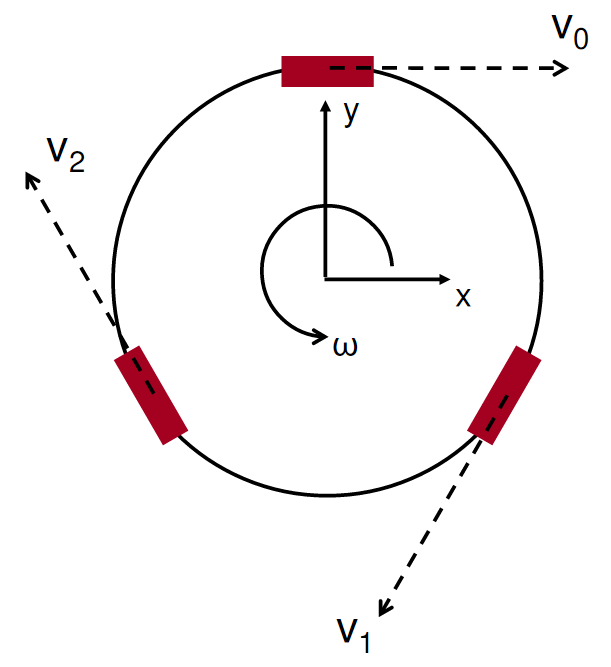
\includegraphics[width=0.25\textwidth]{images/technische_grundlagen/Omniantrieb.png}
	\end{center}
	\caption{Einachsige Lenkung}
	\label{fig:einachsenlenkung}
\end{wrapfigure}
\paragraph{Omni-Antrieb}
Beim Omni-Antrieb kommen omnidirektionale Räder wie Allseitenräder oder Mecanum-Räder zum Einsatz. Durch ihren speziellen Aufbau ist der Roboter in der Lage, sich sowohl auf der Stelle zu Drehen, als auch in alle Richtungen zu bewegen, ohne sich vorher drehen zu müssen. Dies verleiht dem Antrieb eine uneingeschränkte Beweglichkeit in jede Richtungen (x, y und $\omega{}$).
\newline
Der Große Vorteil dieser Antriebsform ist die uneingeschränkte Beweglichkeit. Jedoch birgt diese Art des Antriebs eine gewisse mechanische Komplexität und erfordert eine aufwändige Steuerung.

\newpage
\subsection{\LM}
\LM{} ist eine seit 1988 existierende Produktserie des Spielwarenherstellers \LE{}.\footnote{\citep[vgl.][Das EV3 Roboter Universum, Seite 21]{Scholz.DasEV3}\label{note23}}
\LM{} ermöglicht das Bauen, Programmieren und Steuern verschiedener \LE{} Roboter. Diese Roboter bestehen dabei aus
gängigen \LE{} Teilen die auch in anderen \LE{}-Produkten Verwendung finden, sowie speziellen \LE{}-Komponenten 
wie einer zentralen Steuereinheit, Motoren und Sensoren.
%-------------------------------------------------------------------------------------------------------------------------------------------
%### Subsektion über XXX ###################################################################################################################
%-------------------------------------------------------------------------------------------------------------------------------------------
\subsubsection{Das EV3-System}
Der 2013 erschienene EV3 ist das dritte System der \LM{} Reihe. Die Bezeichnung setzt sich aus EV für Evolution 
und 3 für die dritte Stufe der \LM{}-Serie zusammen.\footref{note23} \\
Im Vergleich zu den Vorgängersystemen verfügt das EV3-System über eine modernere und leistungsfähigere Steuereinheit und auch die anderen elektronischen Komponenten des System wurden an den heutigen Stand der Technik 
angepasst.\footnote{\citep[vgl.][Das EV3 Roboter Universum, Seite 22]{Scholz.DasEV3}\label{note24}}
\medskip
\newline
Die folgende Abbildung \ref{fig:ev3system} zeigt einige der zentralen Komponenten des EV3-Systems, wie die Steuereinheit (EV3-Stein), Motoren und vier Sensoren.
\begin{figure}[ht]
	\centering
	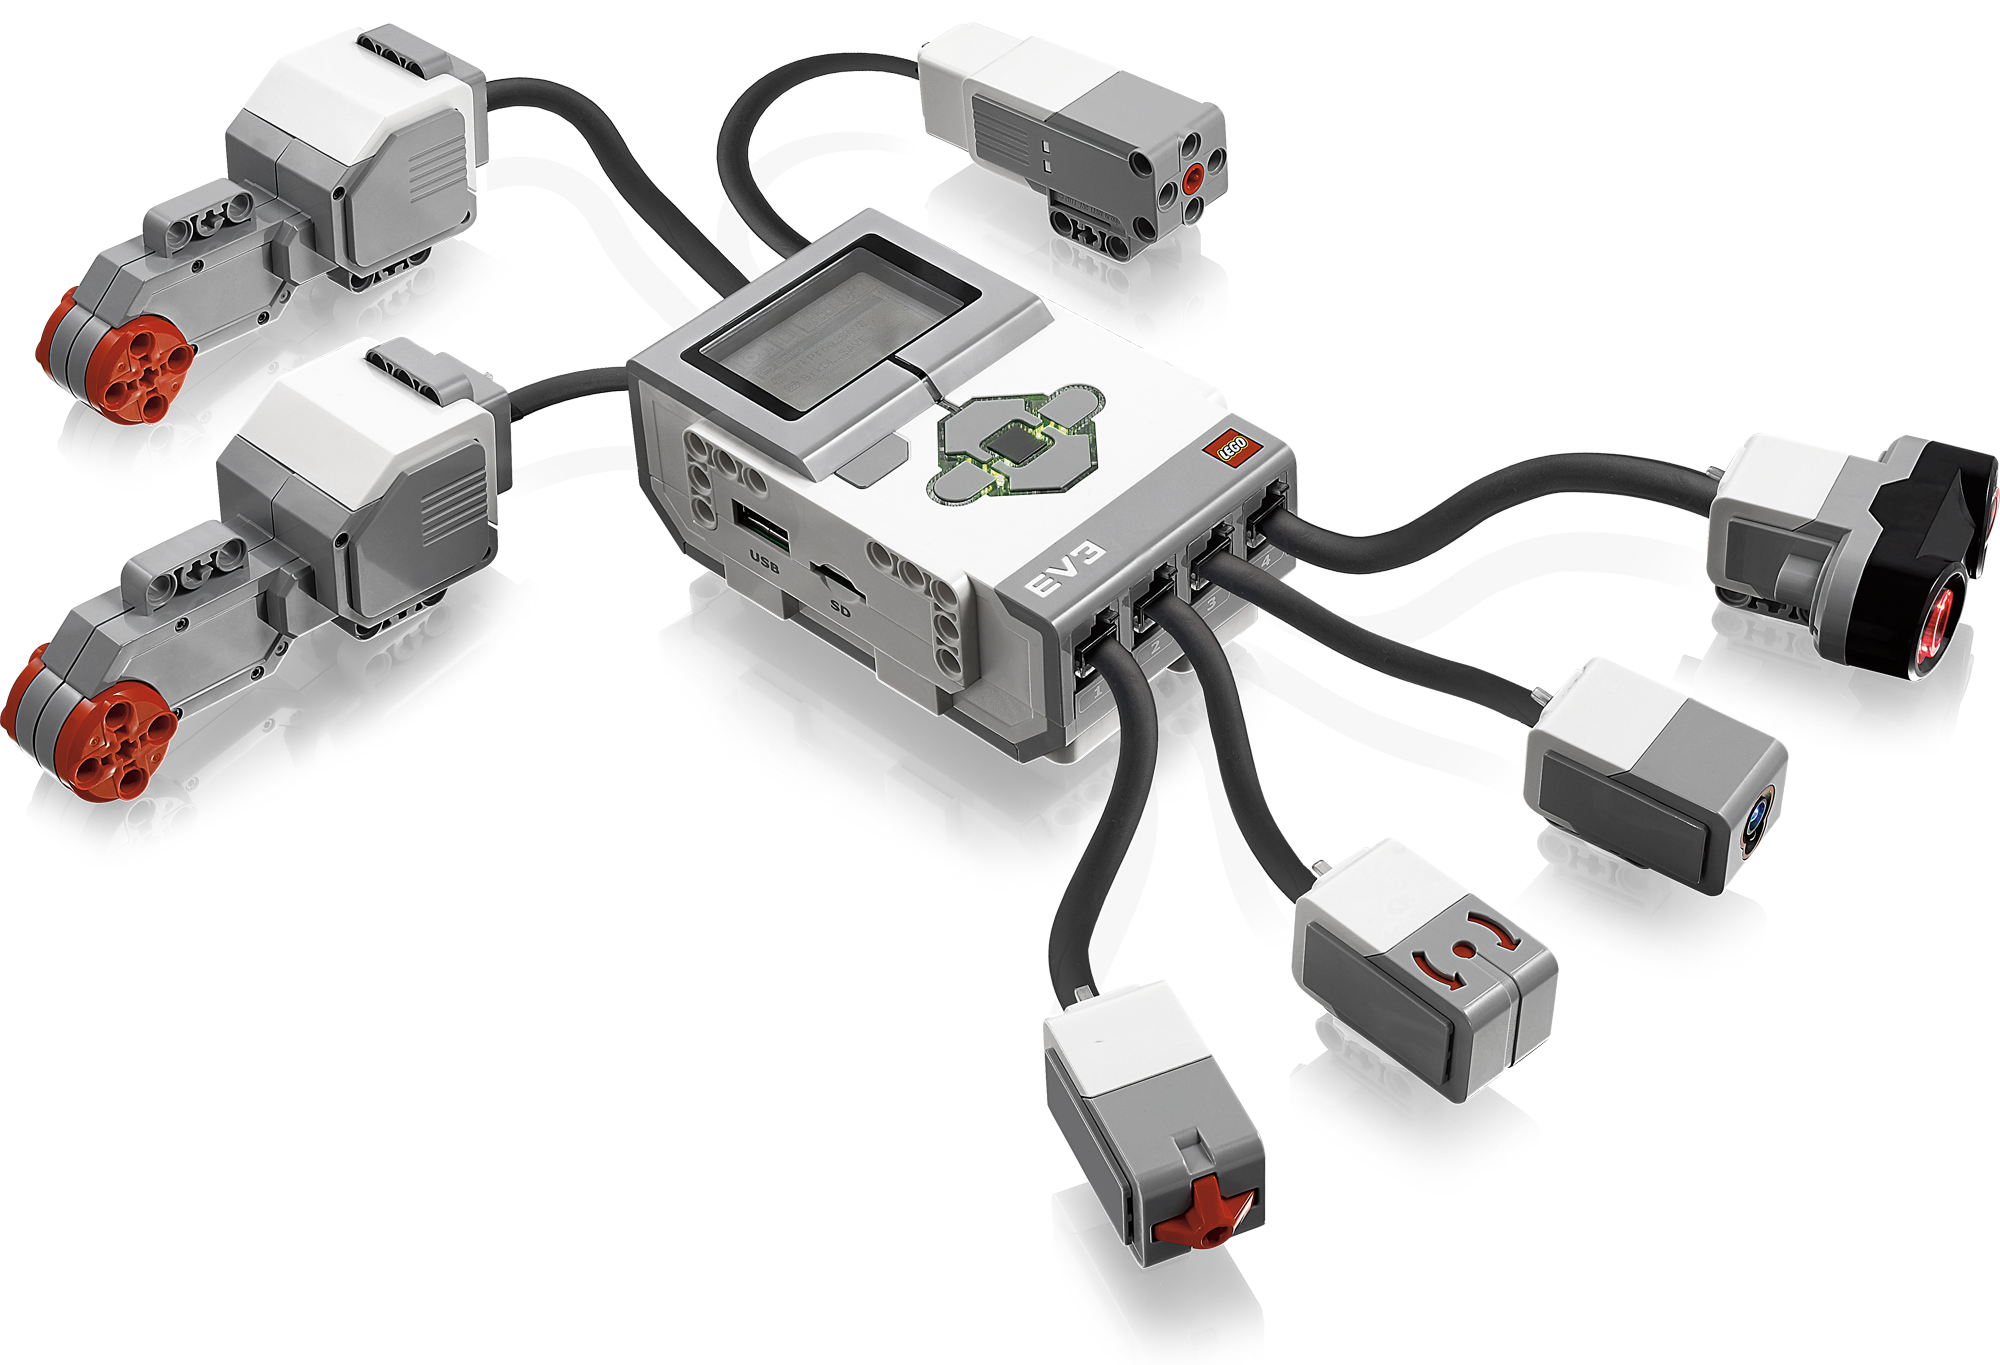
\includegraphics[width=0.90\textwidth]{images/technische_grundlagen/EV3-Overview.png}
	\caption[Zentrale Komponenten des EV3-Systems]{Zentrale Komponenten des EV3-Systems}
	\label{fig:ev3system}
\end{figure}
\newline
Neben den elektronischen Komponenten gehören auch nicht elektronische Teile, wie Verbindungsstücke, Balken und Zahnräder, wie sie aus gängigen \LE{} Produkten bekannt sind, zum EV3-System. Sie bilden die strukturelle und mechanische Grundlage der Roboter.
\medskip
\newline
Im Folgenden wird auf die elektronischen Komponenten des EV3-Systems näher eingegangen, da diese im Projekt eine deutlich größere Relevanz aufweisen.
\subsubsection{Der EV3-Stein (Steuereinheit)}
Die zentrale Komponenten und das Gehirn des LEGO MINDSTORMS EV3-Systems ist die zentrale Steuereinheit, kurz (EV3-)Stein oder auch Brick genannt. Bei ihm handelt es sich um einen Computer, welcher selbständig Programme ausführen kann. Dazu verfügt der EV3-Stein über ein Linux Betriebssystem und eine spezielle Firmware, die wie die auszuführenden Programme auf einem Flash-Speicher liegen.\footnote{\citep[vgl.][Das EV3 Roboter Universum, Seite 21]{Scholz.DasEV3}\label{note25}} \\
Zur Kommunikation mit dem PC verfügt der EV3-Stein über eine USB- sowie Bluetooth-Schnittstelle. Neben der Kommunikation zu einem Computer kann die USB-Schnittstelle auch für den Zusammenschluss mit einem weiteren EV3-Stein (genannt Daisy Chain) genutzt werden.\footref{note25}  \\
Für den Anschluss von Motoren und Sensoren verfügt der EV3-Stein über 8 Ports, an welche die anderen System-Komponenten über Kabel mit RJ12-Steckern angeschlossen werden. 4 der Ports dienen für den Anschluss von
Motoren, die restlichen 4 Ports für die Abfrage von Sensorwerte.\footref{note25} \\
Der EV3-Stein besitzt an der Vorderseite ein LCD-Display zur Anzeige von Texten und Grafiken sowie 6 Knöpfe für die Bedienung durch den Benutzer. Display und Knöpfe dienen zur Bedienung der Firmware sowie zur Tätigung von Einstellungen, können aber ebenso durch Programme angesprochen und ausgewertet werden.\footref{note25}
\medskip
\newline
Die folgende Auflistung zeigt einige Leistungsmerkmale des EV3-Steins.\footnote{\citep[vgl.][Das EV3 Roboter Universum, Seite 23 f., EV3-Programmieren mit Java, Seite 32]{Scholz.DasEV3, Schobel.RobertaEV3Programmieren}\label{note26}}
\begin{itemize}
	\item{Prozessor:} ARM9 32Bit, 300 MHz, 16 MB Flash 64MB RAM
	\item{Betriebssystem:} Linux
	\item{Sensoranschlüsse:} 4x, Analog / Digital bis zu 460,8 Kbit/s
	\item{USB-Schnittstellen:} 2x, für Kommunikation zum PC, Daisy Chain, WiFi-Stick, USB-Speichermedium
	\item{SD-Karten-Lesegerät:} 1x, für MicroSD-Karte bis 32 GB
	\item{User-Interface:} 6 Knöpfe inkl. Beleuchtung
	\item{Display:} LCD Matrix, monochrom, 178 x 128 Pixel
	\item{Kommunikation:} Bluetooth v2.1, USB 2.0 (Kommunikation zum PC), USB 1.1 (Daisy Chain)
\end{itemize}
\subsubsection{Motoren}\label{motoren}
Das EV3-System verfügt über zwei unterschiedliche Motoren, einen großen Motor und einen mittleren Motor. Bei beiden handelt es sich um Servomotoren mit integriertem Rotationssensor, welche von außen angesteuert und abgefragt werden können.\footnote{\citep[vgl.][EV3-Programmieren mit Java, Seite 92]{Schobel.RobertaEV3Programmieren}\label{note27}} Die Motoren lassen sich sehr exakt steuern und ermöglichen so einen synchronen Betrieb mehrerer Motoren.\footnote{\citep[vgl.][Das EV3 Roboter Universum, Seite 29 f.]{Scholz.DasEV3}\label{note28}}
\smallskip
\newline
Die folgende Tabelle zeigt die wichtigsten Eigenschaften der beiden Motoren.
\begin{table}[ht]
	\begin{tabular}{|p{4,5cm}|p{4,0cm}|p{4,0cm}|} \hline
		Eigenschaft / Motortyp		                & Großer Motor         & Mittlerer Motor    \\ \hline
		Winkelgenauigkeit       & 1 $^\circ$           & 1 $^\circ$         \\ \hline
		Umdrehungen    			& 160 bis 170 U/min    & 240 bis 250 U/min  \\ \hline 
		Drehmoment Rotation		& 20 Ncm               & 8 Ncm    			\\ \hline  
		Drehmoment Stillstand 	& 40 Ncm               & 12 Ncm    			\\ \hline  
		Gewicht    				& 76g                  & 36g   		 		\\ \hline
	\end{tabular}
	\centering
	\caption[Eigenschaften der EV3-Motortypen]{Eigenschaften der EV3-Motoren}
\end{table}
\subsubsection{Sensoren}
Zum EV3-System gehören eine Reihe von verschiedenen Sensoren, die es den Robotern ermöglichen Informationen über ihre Umwelt zu sammeln sowie ihre Eigenbewegungen zu erfassen. Im folgenden Abschnitt werden die wichtigsten Sensoren mit ihren Leistungsmerkmalen beschrieben.
\paragraph{Farbsensor}
Der Farbsensor ist ein digitaler Sensor, der dazu dient die Lichtintensität sowie verschiedener Farben zu erkennen. Der Sensor kann sowohl
aktiv, als auch passiv betrieben werden und verfügt dafür über vier unterschiedliche Betriebsmodi:\footnote{\citep[vgl.][EV3-Programmieren mit Java, Seite 101]{Schobel.RobertaEV3Programmieren}\label{note29}}
\begin{itemize}
	\item{Farbmodus (passiv)} - In diesem Modus erkennt der Sensor 7 verschiedenen Farben.
	\item{RGB-Modus (aktiv)} - In diesem Modus sendet der Sensor nacheinander rotes, grünes und Balles Licht aus, je nachdem zu welchem Anteil ein Gegenstand die einzelnen Farben reflektiert wird die Farbe des Gegenstands ermittelt.
	\item{Rotlicht-Modus (aktiv)} - Bei diesem Modus wird Rotlicht ausgesendet und die Intensität des reflektierten Lichts gemessen.
	\item{Umgebungslicht-Modus (passiv)} - Bei diesem Modus wird die Intensität des in das Sensorfenster eindringende Umgebungslichts gemessen.
\end{itemize}
\smallskip
Eigenschaften:
\begin{itemize}
	\item{Erkennung der Farben:} keine Farbe, Schwarz, Blau, Grün, Gelb, Rot, Weiß, Braun
	\item{Abtastrate:} 1.000 Hz
	\item{Entfernung:} 15 bis 50 mm
\end{itemize}
Durch diesen Sensor wird es beispielsweise möglich, den Roboter einer farbigen Linie auf dem Boden folgen zu lassen.
\paragraph{Ultraschallsensor}
Diese aktive Sensor verwendet einen für den Menschen unhörbaren Ultraschall, um die Entfernung von Objekten zu ermitteln. Der Sensor emittiert dazu Ultraschall und misst die Laufzeit der Schallwellen, wenn diese von einem Objekt reflektiert werden, aus der Laufzeit kann dann die Entfernung ermittelt werden. Der Sensor verfügt über zwei unterschiedliche Betriebsmodi:\footnote{\citep[vgl.][Das EV3 Roboter Universum, Seite 32 f.]{Scholz.DasEV3}\label{note30}}
\begin{itemize}
	\item{Messen} - In diesem Modus sendet der Sensor Ultraschall aus, um die Entfernung von Objekten zu ermitteln.
	\item{Scannen} - In diesem passiven Modus emittiert der Sensor selbst keinen Ultraschall, sondern er reagiert auf fremden Ultraschall und kann so einen anderen aktiven Ultraschallsensor erkennen.
\end{itemize}
\smallskip
Eigenschaften:
\begin{itemize}
	\item{Genauigkeit: +/- 1 cm}
	\item{Messbereich: 3 cm bis 250 cm}
\end{itemize}
\paragraph{Berührungssensor}
Der Berührungssensor ist ein einfacher mechanischer Sensor. Wird der Knopf am Ende des Sensors gedrückt wird dies registriert. Trotz der Einfachheit dieses Sensors ist dieser dennoch sehr nützlich, da er beispielsweise die Kollision des Roboters mit einem Hindernis erkennen kann.\footnote{\citep[vgl.][Das EV3 Roboter Universum, Seite 33]{Scholz.DasEV3}\label{note31}}
\paragraph{Kreiselsensor (Gyroskop)}
Der Kreiselsensor ermöglicht es Drehbewegungen um eine Achse über Rotationsgeschwindigkeit und Drehwinkel zu messen. Dadurch wird es möglich die Eigenbewegung des Roboters oder einer Roboterkomponente zu registrieren.\footnote{\citep[vgl.][Das EV3 Roboter Universum, Seite 33]{Scholz.DasEV3}\label{note32}}
\medskip
\newline
Eigenschaften:
\begin{itemize}
	\item{Genauigkeit: +/- 3$^\circ$ (bei einer 90$^\circ$ Drehung)}
	\item{Geschwindigkeit: maximal 440 Grad/Sekunde}
	\item{Abtastrate: 1.000 Hz}
\end{itemize}
\paragraph{Rotationssensor (Integriert)}
Wie bereits im Abschnitt \eqref{motoren} dargelegt verfügen die beiden Motortypen über integrierte Rotationssensoren, die es ermöglichen die Umdrehungen der Motoren auszulesen. Durch diese Sensoren können mittels Odometrie Rückschlüsse über die Bewegung bzw. Position des Roboters geschlossen werden.
\medskip
\newline
Eigenschaften:
\begin{itemize}
	\item{Genauigkeit: 1$^\circ$ }
	\item{Umdrehungen: Motorabhängig}
\end{itemize}
\bigskip
Neben den hier vorgestellten Sensoren existiert noch ein Infrarotsensor, welcher in Verbindung mit einer Infrarotfernsteuerung dazu dient einen EV3-Roboter fernzusteuern.
%### Subsubsektion über XXX ################################################################################################################
\subsubsection{Programmierung}
Für die Programmierung der \LM{} Produkte gibt es eine Reihe unterschiedlicher Programmiersprachen und -umgebungen. Die hauseigene \LE{}-Software zur Programmierung des EV3 richtet sich an Einsteiger. Sie ermöglicht es über eine grafische Oberfläche via vorgefertigter Programmabläufe, welche durch grafische Blöcke repräsentiert werden den EV3 zu programmieren.\footnote{\citep[vgl.][EV3-Programmieren mit Java, Seite 25 f.]{Schobel.RobertaEV3Programmieren}\label{note33}} \\
%cite[vgl.][25\psq]{Roberta}.
Die Abbildung \eqref{tab:ev3motoreneig} gibt einen Überblick über verschiedene für den EV3 verfügbare Programmiersprechen sowie ihre Vor- und Nachteile.
\begin{table}[ht]
	\begin{tabular}{|p{4,5cm}|p{2,0cm}|p{2,0cm}|p{2,0cm}|p{2,0cm}|} \hline
		Eigenschaft / Programmiersprache  & leJOS      & EV3-Software  & RobotC  & NEPO       \\ \hline
		Installation                      & +          & ++            & +       & +++        \\ \hline
		Handhabung    		           	  & +          & ++            & +       & ++         \\ \hline
		Kosten                            & kostenlos  & kostenlos     & 49\$    & kostenlos  \\ \hline
		Einstieg 	                      & 0          & ++            & +       & +++        \\ \hline  
		Funktionsumfang    				  & ++         & +             & ++      & ++         \\ \hline
	\end{tabular}
	\centering
	\newline
	0 = neutral; + = gut; ++ = sehr gut; +++ = hervorragend
	\caption[Eigenschaften der EV3-Motortypen]{Eigenschaften der EV3-Motoren}
	\label{tab:ev3motoreneig}
\end{table}
\newpage
\paragraph{leJOS}
Das LEGO Java Operating System abgekürzt leJOS ist ein Framework, dass es ermöglicht den EV3 mit der Programmiersprache Java zu programmieren. Das leJOS-Projekt wurde 1999 gegründet und sämtliche Komponenten (wie auch Java) sind kostenlos verfügbar.\footnote{\citep[vgl.][EV3-Programmieren mit Java, Seite 21]{Schobel.RobertaEV3Programmieren}\label{note34}} \\
leJOS bietet eine schlanke Java Virtual Machine (JVM) für den EV3-Stein sowie eine Klassenbibliothek mit welcher die Komponenten des EV3 (Motoren, Sensoren etc.) angesprochen werden können. Installiert wird leJOS auf einer bootbaren microSD-Karte und kann anschließend davon gestartet werden, ohne die auf dem EV3 vorhandene LEGO-Software zu löschen oder zu verändern.\footnote{\citep[vgl.][EV3-Programmieren mit Java, Seite 23]{Schobel.RobertaEV3Programmieren}\label{note35}} \\
Durch leJOS ist es möglich den EV3 mit Hilfe der Hochsprache Java zu programmieren, womit eine mächtige Programmiersprache zur Verfügung steht und die Vorteile der Objektorientierung für den EV3 genutzt werden können.
leJOS bietet eine umfangreiche Klassenbibliothek sowie gut dokumentierte API was unter anderem die Integration von weiteren Sensoren etc. erleichtert.\footref{note35}
Im folgenden sind einige Features die leJOS bietet aufgelistet:
\begin{itemize}
	\item{Objektorientierte Programmierung mit Java}
	\item{Die meisten Klassen der Pakete \code{java.lang}, \code{java.util} und \code{java.io}}
	\item{Rekursion}
	\item{Synchronisation}
	\item{Multithreading}
	\item{Exceptions}
	\item{Vollständige Bluetooth Unterstützung}
	\item{Umfangreiche Klassenbibliothek zum Steuern und Auslesen der EV3-Komponenten}
	\item{High-Level-Robotik-Tasks (Navigation, Lokalisation etc.)}
\end{itemize}

\newpage
\subsection{\gls{app} Entwicklung} %Simon ca. 8

\begin{wrapfigure}{r}{0.45\textwidth}
	\begin{center}
		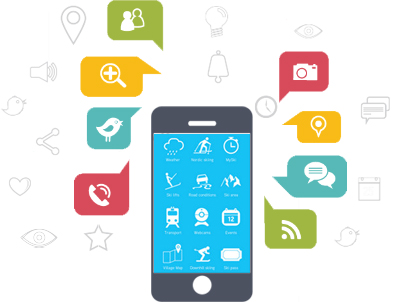
\includegraphics[width=0.4\textwidth]{images/technische_grundlagen/App-Development.jpg}
	\end{center}
	\caption{App-Entwicklung \cite{Nethority.Web&App}}	
	\label{fig:appentwicklung}
\end{wrapfigure}

Eine \gls{app} ist ein ausführbares Programm für mobile Geräte, wie Smartphones oder Tablets. Um eine \gls{app} für ein mobiles Gerät zu entwickeln, müssen vor Start der Entwicklung Anforderungen definiert sein, damit die Software spezifisch angepasst werden kann. Je nach Art der Anforderungen die an das System gestellt werden, bestehen verschiedene Möglichkeiten der Entwicklung. Allgemein kennt die \gls{app} Entwicklung drei verschiedene Arten, die Native-, Web- und Hybride-Entwicklung, siehe Abschnitt \eqref{native}, \eqref{web} und \eqref{hybride}. Dabei werden verschiedene \glspl{framework} verwendet, um mit unterschiedlichen Programmiersprachen den Aufbau der Logik zu beschreiben. Eine \gls{app} besteht immer aus zwei Teile, dem \gls{ui}, das meist mit einer \gls{xml} oder \gls{html} und \gls{css} ähnlichen Sprache beschrieben wird und dem Programmcode, der sich auf viele Klassen verteilt und die Funktionalitäten der \gls{app} beschreiben.

\subsubsection{Native \glspl{app}}\label{native}

In der Entwicklung von nativen \glspl{app} werden die direkten Ressourcen des Gerätes verwendet. Dazu gehört die Laufzeitumgebung des Betriebssystems, Bibliotheken und Hardwareschnittstellen. Der Vorteil von einer nativen Entwicklung liegt hauptsächlich darin, dass diese für das Betriebssystem optimiert ist und die vorhandenen Schnittstellen genutzt werden können, um komplexe und rechenintensive Anwendungen zu ermöglichen.\footnote{\citep[vgl.][Unterschiede und Vergleich native Apps vs. Web Apps]{DanielWurstl.Unterschiedeund}\label{note36}}\\
Vertreter diese Entwicklung finden sich für verschiedene Betriebssysteme. Der populärste unter ihnen ist bei weitem Android mit einer nativen Java Entwicklung über Android Studio von Google. Native \glspl{app} besitzt aktuell den höchsten Marktanteil und eine entsprechende Popularität unter Entwicklern und Nutzern.

\subsubsection{Web \glspl{app}}\label{web}

Die Entwicklung von web \glspl{app} arbeitet mit systemübergreifenden Ressourcen und greift auf gängige Webtechnologien, wie \gls{html}, \gls{css} und \gls{javascript} zurück. Die \gls{app} wird hierbei nicht wie normale Anwendungen direkt auf dem System des Gerätes ausgeführt, sondern kommt in dessen Browser zur Ausführung. Der Vorteil hierbei ist vor allem, dass diese Art von \gls{app} auf allen Betriebssystemen lauffähig ist und direkt über das Internet veröffentlicht und aktualisiert werden kann, jedoch wird eine stabile Internetverbindung vorausgesetzt.\footref{note36}\\
Diese Entwicklung besitzt viele Vertreter mit der Unterstützung diverser \glspl{framework}. Das populärste unter ihnen ist aktuell AngularJS von Google, was auf \gls{javascript} basiert. In Kombination mit anderen Webtechnologien, wie \gls{html} und \gls{css} lassen sich perfomante Web-\glspl{app} entwickeln.

\subsubsection{Hybride \glspl{app}}\label{hybride}

Die Entwicklung von hybriden \glspl{app} vereinigt die native- und webbasierte Entwicklung. Sie besteht dabei aus einem nativen Rahmen, in der eine Web-\gls{app} zur Ausführung kommt, diese besitzt entsprechende Zugriffsrechte auf Hardwareschnittstellen, um diese mit \glspl{api} anzusprechen.\footnote{\citep[vgl.][Native App, Web App und Hybrid App im Überblick]{PetraRiepe.NativeApp}\label{note37}}\\
Diese Entwicklung ist aktuell noch sehr jung, jedoch treten hier bereits verschiedene Vertreter hervor. Der populärste unter ihnen ist Ionic von Drifty, welches auf Apache Cordova als Basis zurückgreift. In Kombination mit AngularJS, \gls{typescript} und anderen Webtechnologien lässt sich die hybride \gls{app} entwickeln und auf einem beliebigen Gerät unter einem nativen Browser ausführen. Hybride \glspl{app} unterstützten dabei verschiedene Betriebssystem, wie Android, iOS und Windows. Diese \glspl{app} können dabei meist nicht nur mobil, sondern unter anderem auf weiteren Systemen, wie stationäre zum Beispiel Desktop Rechner bereitgestellt werden.

\subsubsection{Plattformübergreifende \glspl{app}}

Um die Entwicklung von \glspl{app} einfach zu gestalten, verwenden immer mehr Entwickler die Form der plattformübergreifenden Entwicklung. Dadurch lässt sich die \gls{app} unabhängig des Betriebssystem entwickeln und kann somit eine größere Menge von Nutzern erreichen. Diese Entwicklung greift dabei meist auf plattformübergreifende Konzepte, wie eine native Laufzeitumgebung oder einen nativen Browser zurück, um darin die \gls{app} auszuführen. Der große Vorteil dieser \glspl{app}, liegt in der Wiederverwendbarkeit des Quellcodes und der verbesserten Wartbarkeit, da hier lediglich ein Projekt gewartet werden muss und der Quellcode für viele Betriebssysteme übernommen werden kann. Zur plattformübergreifenden Entwicklung wurden in den letzten Jahre viele Ansätze mit verschiedenen \glspl{framework} entwickelt. Beispiele hierfür sind Ionic, Unity, Qt oder Xamarin.\\
\newpage

\subsubsection{Xamarin}

\begin{wrapfigure}{r}{0.3\textwidth}
	\begin{center}
		
\includegraphics[width=0.25\textwidth]{images/technische_grundlagen/xamarin.png}
	\end{center}
	\caption{Xamarin \cite{Xamarin}}
	\label{fig:xamarin}
\end{wrapfigure}

Xamarin ist ein \gls{framework} zur Entwicklung von nativen, plattformübergreifenden \glspl{app}. Es basiert auf dem Mono Projekt, siehe Abschnitt \eqref{mono}, um damit auf verschiedenen Betriebssysteme, wie Android, iOS, Windows und Windows Phone ausgeführt werden zu können. Um nativen Quellcode auf den verschiedenen Systemen auszuführen, setzt Xamarin auf verschiedene Softwarekomponenten, um aus einem mit .NET entwickelten Projekt nativen Quellcode zu erzeugen.\\
Für iOS Systeme verwendet Xamarin den \gls{aot} Compiler, um aus einem Xamarin.iOS Projekt, \gls{arm} Maschinencode zur erzeugen, der entsprechend schnell auf dem System ausgeführt werden kann.\footnote{\citep[vgl.][Introduction to Mobile Development - Xamarin]{Xamarin.Introductionto}\label{note38}} Bei Android hingegen wird der Quellcode in \gls{il} übersetzt, eine plattformübergreifende Assemblersprache, die durch das .NET \gls{framework} zur Ausführung gebracht wird. Die Übersetzung in \gls{il} geschieht mittels \gls{jit}, um zur Laufzeit Maschinencode für das entsprechende Gerät zu erzeugen.\footref{note38} Damit dies bewerkstelligt werden kann, nutzt Xamarin zur Laufzeit Softwarekomponenten, die bestimmte Prozesse, wie Speicherverwaltung und Plattformoperationen verwalten.\\
Für eine effiziente Entwicklung bringt Xamarin eine große Bandbreite von Funktionalitäten für einen Entwickler. Beispiele sind dafür Bibliotheken, eine Test Cloud, sowie eine Unterstützung von nativen Bibliotheken, beispielsweise für \gls{java} oder \gls{objectivc}. Um mit Xamarin zu entwickeln, gibt es aktuell verschiedene Möglichkeiten auf unterschiedlichen Betriebssystemen. Einerseits kann mit Xamarin Studio auf einem OSX-System, oder mit Visual Studio auf Windows und Linux entwickelt werden.\\
Wie viele andere \glspl{framework}, bietet auch Xamarin für verschiedene Zwecke nützliche \glspl{template}, die jeweils andere Nutzen besitzen. Die Entwicklung der \gls{app} baut dabei vor allem auf zwei Hauptkomponenten von Bibliotheken, den Shared Projects und Protable Class Libraries.

\newpage
\begin{wrapfigure}{r}{0.55\textwidth}
	\begin{center}
		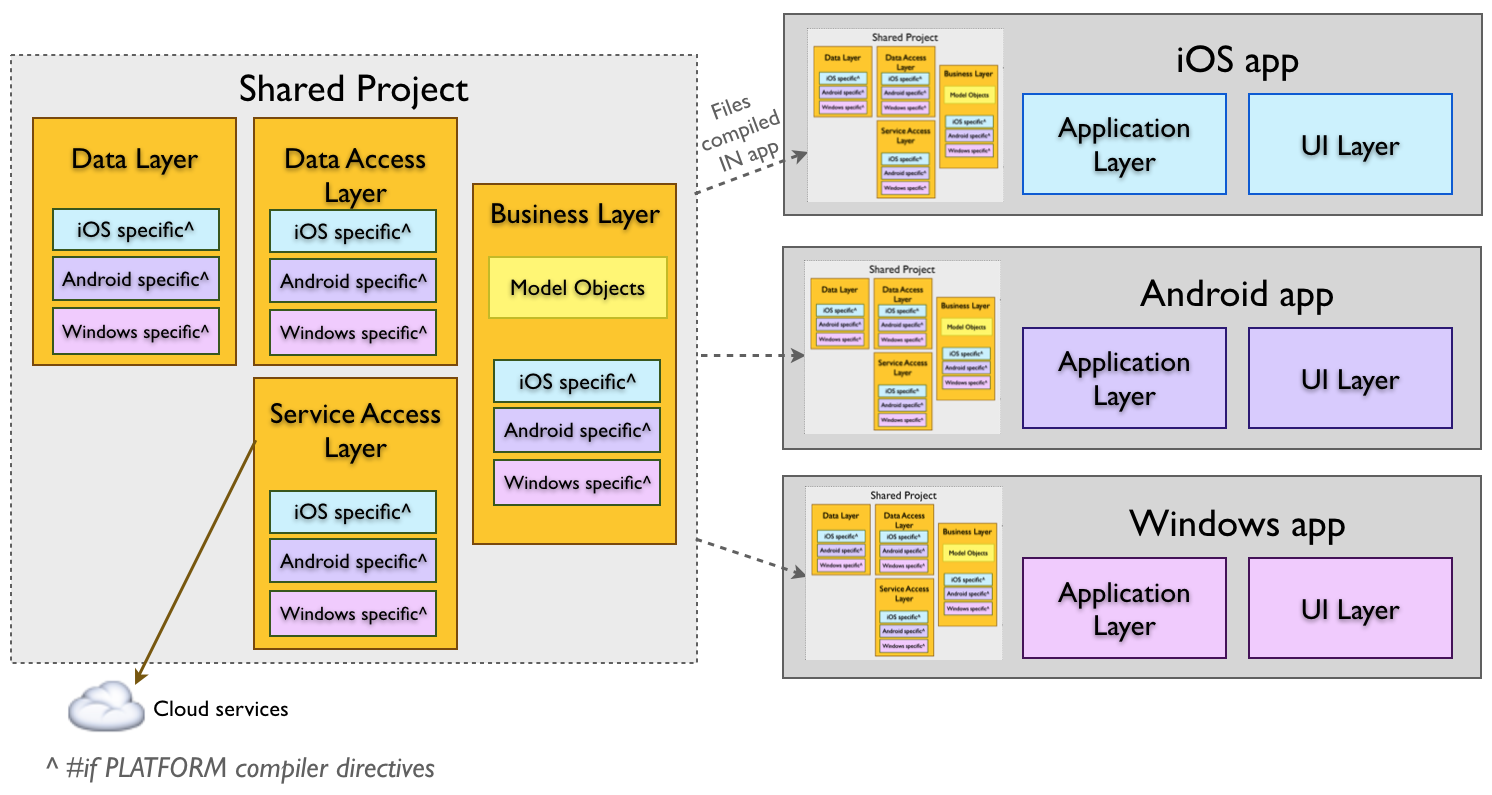
\includegraphics[width=0.5\textwidth]{images/technische_grundlagen/SharedAssetProject.png}
	\end{center}
	\caption{Shared Project \cite{Xamarin.SharedProjects}}
	\label{fig:shared}
\end{wrapfigure}

\paragraph{Shared Projects}

ermöglichen dem Entwickler Quellcode für verschiedene Plattformen zu entwickeln, wobei die plattformspezifischen Projekte das entsprechende Shared Project referenzieren. Somit besitzt diese Projektart keinen direkten Output, sondern kopiert den Quellcode entsprechend in das zu bauende Projekt, siehe Abbildung \eqref{fig:shared}.\footnote{\citep[vgl.][Shared Projects - Xamarin]{Xamarin.SharedProjects}\label{note39}} Der Hauptunterschied zu Standardprojekten liegt vor allem darin, dass ein Shared Project keine Abhängigkeiten haben darf und daher lediglich als Referenz für andere Projekte dienen kann.

\begin{wrapfigure}{r}{0.55\textwidth}
	\begin{center}
		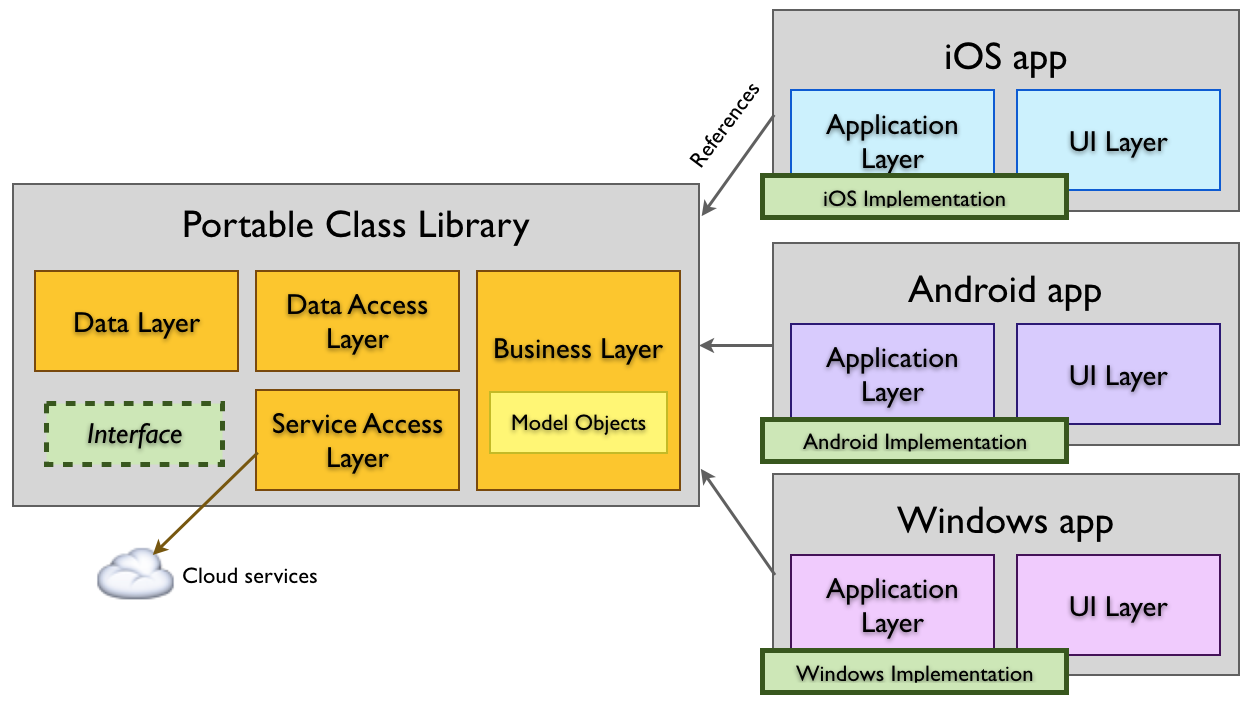
\includegraphics[width=0.5\textwidth]{images/technische_grundlagen/PortableClassLibrary.png}
	\end{center}
	\caption{Portable Class Library \cite{Xamarin.PortableClass}}
	\label{fig:portable}
\end{wrapfigure}

\paragraph{Protable Class Libraries}

ermöglichen dem Entwickler die Implementierung von plattformübergreifenden Bibliotheken, aus denen \glspl{dll} erzeugt werden können. Das Besondere an Portable Class Libraries ist dabei, dass die Plattformen spezifisch ausgewählt werden können, wobei auf die Unterstützung verschiedener Betriebssysteme zu achten ist, siehe Abbildung \eqref{fig:pcl_support}.\footnote{\citep[vgl.][Introduction to Portable Class Libraries - Xamarin]{Xamarin.PortableClass}\label{note40}} Eine Portable Class Library besitzt darüber hinaus verschiedene Vor- bzw. Nachteile, die für oder gegen ihre Nutzung sprechen.\\

\begin{figure}[h]
	\begin{center}
		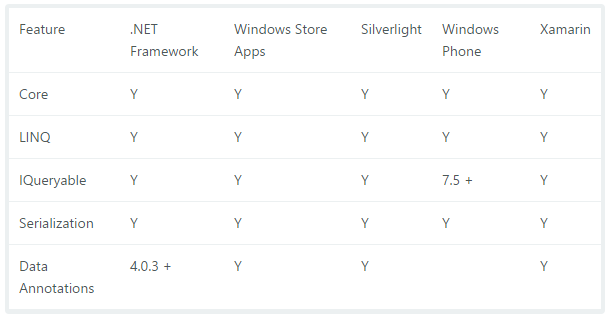
\includegraphics[width=0.5\textwidth]{images/technische_grundlagen/pclSupport.png}
	\end{center}	
	\caption{Unterstützung Portable Class Library \cite{Xamarin.PortableClass}}
\end{figure}

\newpage
\noindent
Vorteile:
\begin{itemize}
	\item Implementierung von zentralem Quellcode
	\item Einfaches Refactoring
	\item Referenzierung von Anwendungen
\end{itemize}
\noindent
Nachteile:
\begin{itemize}
	\item Keine Referenzierung von plattformspezifischen Quellcode
	\item Keine Standardbibliotheken vorhanden
\end{itemize}

\begin{wrapfigure}{r}{0.45\textwidth}
	\begin{center}
		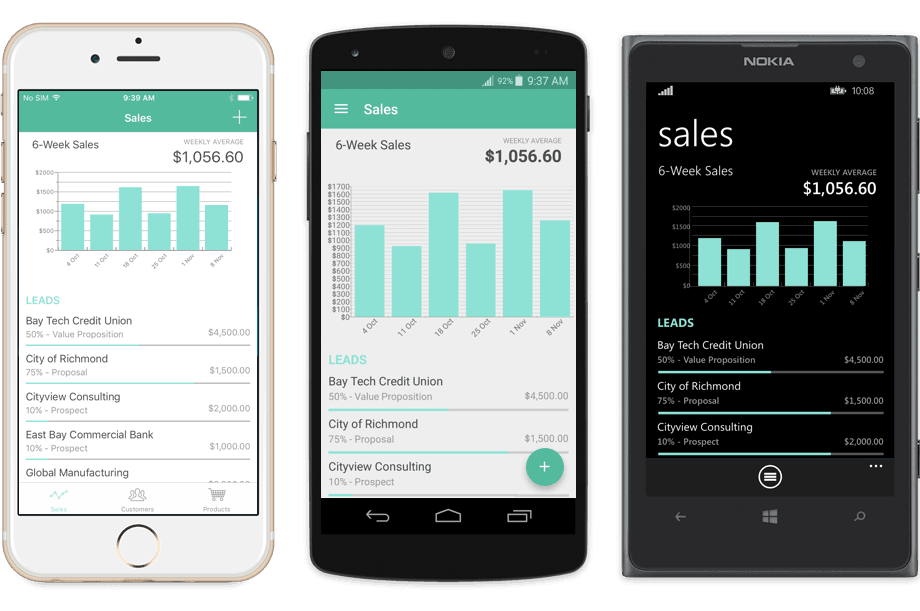
\includegraphics[width=0.4\textwidth]{images/technische_grundlagen/forms.png}
	\end{center}	
	\caption{Design Xamarin.Forms \cite{Xamarin.Builda}}
	\label{fig:forms}
\end{wrapfigure}

\paragraph{Xamarin.Forms} ist ein plattformübergreifendes \gls{ui} Werkzeug zur Implementierung eines nativen \gls{gui} durch \gls{xaml}, siehe Abbildung \ref{fig:forms}. Dieses basiert auf den typischen \gls{xml} Strukturrichtlinien, womit sich die verschiedenen Elemente als klaren, übersichtlichen Text darstellen lassen, siehe Abbildung \ref{fig:xaml}. Zur Strukturierung des Designs bietet Xamarin verschiedene Arten von Seiten-, Layout- und Navigationsprinzipien, welche durch Xamarin.Forms auf die nativen Elemente zurückgreifen. Damit lässt sich durch Xamarin.Forms native Designs schaffen, welche plattformübergreifend in Android, iOS und Windows angewendet werden können. Die vorhandenen Designs stellen dabei Klassen dar, die vom Entwickler entsprechend verwendet, oder bei Bedarf durch eigene Implementierungen angepasst werden können.\\

\begin{figure}[h]
	\begin{center}
		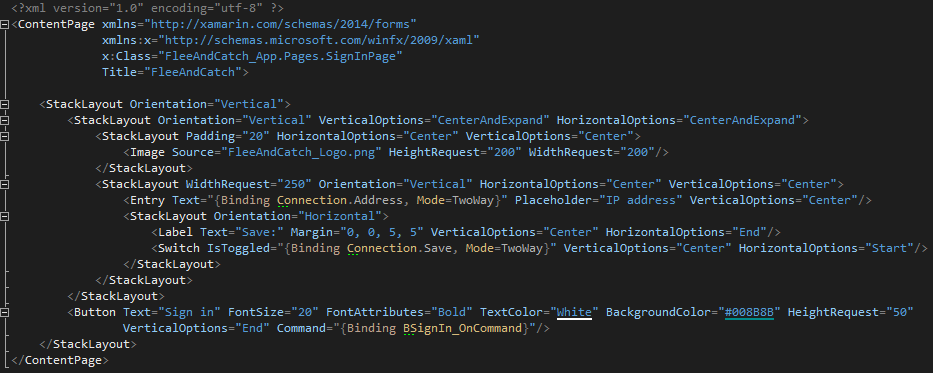
\includegraphics[width=0.7\textwidth]{images/technische_grundlagen/xaml.png}
	\end{center}	
	\caption{SignInPage in \acrshort{xaml}}
	\label{fig:xaml}
\end{figure}

\newpage
\noindent
Xamarin.Forms setzt mit seinem Layout auf bekannte Designprinzipien, welche bereits in anderen Frameworks, wie .NET vorzufinden sind, siehe Abbildung \ref{fig:layout} und \ref{fig:pages}. Diese können in drei Kategorien eingeteilt werden, einerseits die eigentliche Seite, die in verschiedene \glspl{ui} dargestellt werden können und somit die Nutzerinteraktion beeinflussen. Andererseits das Layout, welches die Darstellung der vorhandenen Elemente regelt und den Pages, die für die Navigation unter den einzelnen Seiten zuständig sind. Dem Entwickler sind dabei keinerlei Grenzen gesetzt, wobei dieser sämtliche zur Verfügung stehenden Ressourcen miteinander kombinieren kann.

\begin{figure}[h]
	\begin{center}
		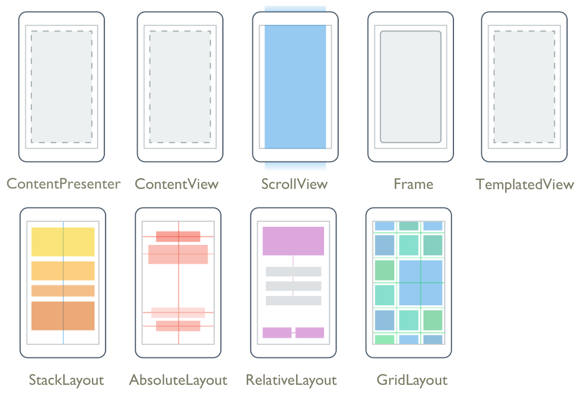
\includegraphics[width=0.8\textwidth]{images/technische_grundlagen/layout.png}
	\end{center}	
	\caption{Xamarin.Forms Layouts \cite{Xamarin.Xamarin.FormsLayouts}}
	\label{fig:layout}
\end{figure}

\noindent

\begin{figure}[h]
	\begin{center}
		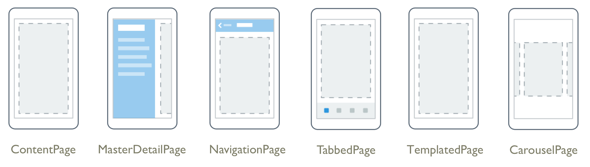
\includegraphics[width=0.8\textwidth]{images/technische_grundlagen/pages.png}
	\end{center}	
	\caption{Xamarin.Forms Pages \cite{Xamarin.Xamarin.FormsPages}}
	\label{fig:pages}
\end{figure}

\newpage
\subsubsection{Mono}\label{mono}

\begin{wrapfigure}{r}{0.3\textwidth}
	\begin{center}
		
\includegraphics[width=0.25\textwidth]{images/technische_grundlagen/mono.png}
	\end{center}
	\caption{Mono \cite{Mono.MonoProject}}
	\label{fig:mono}
\end{wrapfigure}

Mono ist ein Open-Source-Framework, das auf dem .NET Framework von Microsoft basiert. Die Implementierung von Mono greift dabei auf die Standards von .NET für die Programmiersprache \gls{csharp}, sowie die \gls{cli} zurück.\footnote{\citep[vgl.][About Mono]{MonoProject.AboutMono}\label{note41}} Dies ermöglicht Entwicklern die Erstellung von plattformübergreifenden Anwendungen, welche mittels einer zur Verfügung gestellten Laufzeitumgebung auf verschiedenen Systemen ausgeführt werden können.\\
Um Anwendungen auf verschieden Systemen auszuführen, nutzt Mono verschiedene Komponenten. Dazu gehört an vorderster Stelle ein Compiler, um den erstellten Quellcode in die jeweilige Maschinensprache zu übersetzen. Die Übersetzung findet dabei in Kooperation mit der Mono Runtime statt, welche die entsprechende Infrastruktur zur Ausführung der Anwendung bereitstellt. Für eine effiziente Entwicklung stellt Mono zwei Bibliotheken zur Verfügung, einerseits die .NET Class Library, die die Grundelemente von .NET enthält, sowie die Mono Class Library mit zusätzlichen Funktionen für plattformübergreifende Anwendungen.\\
Im Vergleich mit anderen Frameworks sprechen verschiedenen Vorteile für die Nutzung von Mono. Der Hauptgrund für die Nutzung liegt vor allem in der Popularität von .NET, da dies auf den meisten Rechnern zur Verfügung steht, oder installiert werden kann. Ein großer Nutzen stellt die High-Level-Programmierung dar, welche eine Implementierung mit einer Laufzeitumgebung ermöglicht, die Funktionen wie Speicherverwaltung selbst organisiert. Durch Verwendung der \gls{clr} kann der Entwickler seine übliche Programmiersprache verwenden und ist unabhängig vom bestehenden System.

\subsubsection{.NET Framework}\label{net}

Das .NET Framework dient zur Entwicklung sowie Ausführung von Anwendungen, die mit Programmiersprachen implementiert sind, welche auf den Standards von .NET basieren. Es besteht aus verschiedenen Komponenten, wobei der Kern des Frameworks in der \gls{clr} liegt.\footnote{\citep[vgl.][Overview of the .NET Framework]{Microsoft.Overviewof}\label{note42}} Diese ist verantwortlich für die Laufzeitumgebung und somit für die Ausführung der Anwendungen, indem es die bereitgestellten Ressourcen des Systems nutzt.
\newpage
\begin{wrapfigure}{r}{0.45\textwidth}
	\begin{center}
		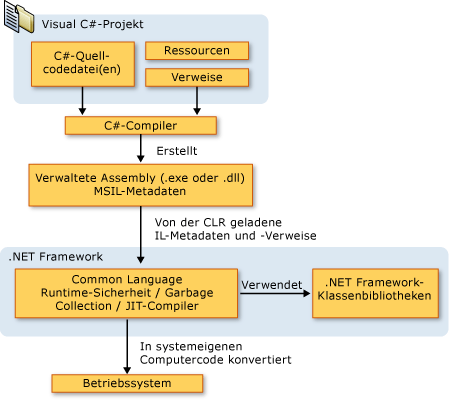
\includegraphics[width=0.4\textwidth]{images/technische_grundlagen/net_aufbau.jpeg}
	\end{center}
	\caption{.NET Framework Ausführung \cite{Microsoft.Introductionto}}
	\label{fig:net}
\end{wrapfigure}

\noindent
Die \gls{clr} führt zur Laufzeit, je nach System, verschiedene Aktionen aus, um die entsprechende Anwendung auszuführen. Der allgemeine Ablauf ist dabei folgender: Der Quellcode wird in die \gls{clr} geladen und nach entsprechenden Sicherheitsanforderungen des Systems überprüft.\footref{note42} Anschließend wird er durch eine \gls{jit} Kompilierung in einen \gls{il}-Quellcode konvertiert, um diesen nativ auf dem System ausführen zu können.\footref{note7} Der \gls{il}-Quellcode setzt dabei auf die gesetzten Standards der \gls{cli} auf, die eine sprach- und plattformunabhängige Entwicklung von Anwendungen ermöglicht.\footref{not42}\\
Das .NET Framework bietet zusätzlich zur unabhängigen Entwicklung verschiedene unterstützende Komponenten. Die wichtigste unter ihnen ist die .NET Class Library. Diese unterstützt den Entwickler mit einer Sammlung bereits implementierten Quellcodes, wie Klassen und entsprechenden Zugang zu systemnahen Schnittstellen. Mit dem .NET Framework lässt sich eine große Bandbreite von Anwendungen entwickeln, von Konsolenanwendungen, über grafischen Oberflächen, bis hin zu Webanwendungen.\\

\begin{figure}[h]
	\centering
	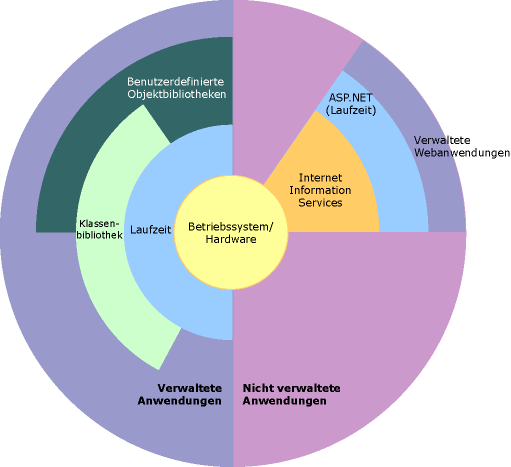
\includegraphics[width=0.65\textwidth]{images/technische_grundlagen/clr.png}
	\caption{Common Language Runtime \cite{Microsoft.Overviewof}}
	\label{fig:clr}
\end{figure}

\subsection{TCP-Kommunikation}
Das \gls{tcp} ist ein Transportprotokoll und ermöglicht eine Datenaustausch zwischen kommunizierenden Anwendungsinstanzen in einer Ende-zu-Ende-Beziehung. \gls{tcp} ist als Transportprotokoll in der vierten Schicht des \gls{osi}-Modells angesiedelt und basiert auf dem \gls{ip} mit dem es zusammen als Namensgeber der TCP/IP-Protokollfamilie (Internetprotokollfamilie) dient.
\gls{tcp} ist ein offenes, frei verfügbares und weit verbreitetes Protokoll. Als Mitglied der Internetprotokollfamilie ist \gls{tcp} neben \gls{udp} das Transportprotokoll, auf dem die meisten Anwendungen im Internet basieren.\footnote{\citep[vgl.][Grundkurs Datenkommunikation, Seite 189]{Mandl.GrundkursDatenkommunikation}\label{note43}}
\subsubsection{Gundlegendes}
Als verbindungsorientiertes Protokoll sorgt TCP für die Erzeugung und Erhaltung einer gesicherten Ende-zu-Ende-Verbindung zwischen zwei Anwendungsprozessen. TCP arbeitet paketvermittelt d.h. überträgt Daten Paketweise und ist ein zuverlässiges Protokoll. Durch diese Eigenschaften stellt TCP sicher, dass Daten
\begin{itemize}
	\item{nicht verloren gehen}
	\item{nicht verändert werden}
	\item{nicht dupliziert werden}
	\item{in der richtigen Reihenfolge eintreffen}
\end{itemize}
Zur Gewährleistung einer vollständigen Übertragung sowie der Integrität der gesendeten Daten nutzt TCP Prüfsummen, Bestätigungen, Zeitüberwachungs- und Nachrichtenwiederholungsmechanismen sowie Sequenznummern für die Reihenfolgeüberwachung und das Sliding Windows Prinzip zur Flusskontrolle.\footnote{\citep[vgl.][Grundkurs Datenkommunikation, Seite 190]{Mandl.GrundkursDatenkommunikation}\label{note44}}
\newline
TCP nutzt prinzipiell folgende Protokollmechanismen:
\begin{itemize}
	\item{Drei-Wege-Handshake-Verbindungsauf- und -abbau}
	\item{Positives, kumulatives Bestätigungsverfahren mit Timerüberwachung für jede Nachricht}
	\item{Implizites negatives Bestätigungsverfahren (NAK-Mechanismus): Bei drei ankommenden Duplikat-ACK-PDUs wird beim Sender das Fehlen des folgenden Segments angenommen. Ein sog. Fast-Retransmit-Mechanismus führt zur Neuübertragung des Segments, bevor der Timer abläuft.}
	\item{Pipelining}
	\item{Go-Back-N zur Übertragungswiederholung}
	\item{Fluss- und Staukontrolle}
\end{itemize}
\subsubsection{Nagle-Algorithmus}
Nagle-Algorithmus (RFC 896 und RFC 1122) ist ein Algorithmus, der der Optimierung dient und der bei allen TCP-Implementierungen verwendet wird. Der Nagle-Algorithmus versucht aus Optimierungsgründen zu verhindern, dass viele kleine Nachrichten gesendet werden, da dies schlecht für die Netzauslastung ist.\footnote{\citep[vgl.][Grundkurs Datenkommunikation, Seite 198]{Mandl.GrundkursDatenkommunikation}\label{note45}} \newline
Dazu werden mehrere Nachrichten zusammengefasst und gebündelt versendet, dies geschieht nach folgendem Prinzip:
\begin{itemize}
	\item{Erhält der \gls{tcp}-Endpunkt Daten vom Anwendungsprozess wird zunächst nur das erste Datenpaket gesendet und die restlichen Daten werden im Sendepuffer gesammelt.}
	\item{Danach werden weitere Daten so lange im Sendepuffer gesammelt bis alle zuvor gesendeten Datenpakete vom Empfänger bestätigt wurden oder so viele Daten im Sendepuffer liegen, dass die einstellte Segmentgröße erreicht ist und ein volles Datenpaket gesendet werden kann.}
\end{itemize}
Dieses Verfahren sorgt zwar für eine gute Netzauslastung, da das Verhältnis von Nutzdaten zu Overhead (\gls{tcp}-Header etc.) steigt, jedoch ist dies nicht für alle Anwendungsszenarien optimal, da es die Latenz erhöht. Insbesondere bei Anwendungen die eine unmittelbare Antwort der Gegenstelle benötigen wie \gls{ssh}- oder Telnet-Anwendung sorgt dies für Verzögerungen. In diesem Fall ist es besser den Nagle-Algorithmus auszuschalten.\footnote{\citep[vgl.][Grundkurs Datenkommunikation, Seite 198 f.]{Mandl.GrundkursDatenkommunikation}\label{note65}}
\subsubsection{Kommunikationsablauf}
Da es sich bei \gls{tcp} um ein verbindungsorientiertes Protokoll handelt gliedert sich die Kommunikation in drei Phasen: Verbindungsaufbau, Datenaustausch und Verbindungsabbau. Bevor Daten übertragen werden können, muss die Verbindung durch den Verbindungsaufbau initiiert und nach Beendigung der Datenübertragung wieder abgebaut werden. 
\paragraph{Client \& Server}
Der Verbindungsaufbau einer Kommunikation erfolgt bei \gls{tcp} nach dem Client-/Server-Paradigma, d.h. einer der Teilnehmern agiert als Server und wartet auf einen Verbindungsaufbau durch den Client, welchen der andere Teilnehmern darstellt. \newline
Nach dem Verbfindungsaufbau haben die beiden Rollen jedoch keine Bedeutung mehr und die beide Teilnehmern sind sowohl bei der Datenübertragung, als auch beim Verbindungsabbau gleichberechtigt.
\paragraph{Verbindungsaufbau}
Der Verbindungsaufbau bei \gls{tcp} basiert auf dem Three-Way-Handshake. Dabei schickt der Client einen Verbindungswunsch (SYN) an den Server. Der Server bestätigt den Erhalt der Nachricht (ACK) und äußert seinerseits einen Verbindungswunsch (SYN), welchen der Client nach Erhalt der Nachricht bestätigt (ACK). Nach Ablauf dieses gegenseitigen Anfrage- und Bestätigungsvorgangs ist die Verbindung initiiert und der Datenaustausch zwischen den Teilnehmern kann beginnen [EK].\footnote{\citep[vgl.][TCP-Kommunikation]{Schnabel.TCPKommunikation}\label{note66}}
\begin{figure}[h]
	\centering
	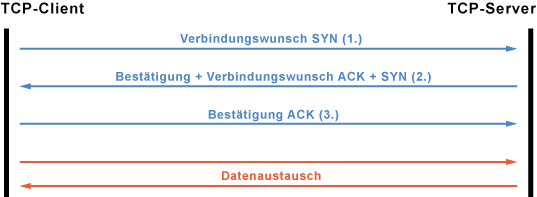
\includegraphics[width=0.8\textwidth]{images/Verbindungsaufbau.png}
	\caption[TCP Verbindungsaufbau]{TCP Verbindungsaufbau \cite{Schnabel.TCPKommunikation}}
	\label{fig:<Sprungmakre>}
\end{figure}
\paragraph{Datenaustausch}
\begin{figure}[h]
	\centering
	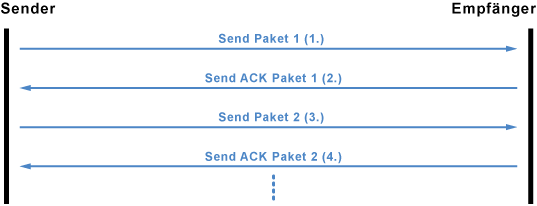
\includegraphics[width=0.8\textwidth]{images/Datenaustausch.png}
	\caption[TCP Datenaustausch]{TCP Datenaustausch \cite{Schnabel.TCPKommunikation}}
	\label{fig:<Sprungmakre>}
\end{figure}
\paragraph{Verbindungsabbau}
\begin{figure}[h]
	\centering
	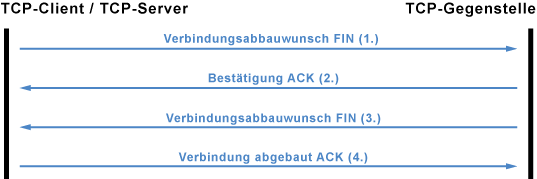
\includegraphics[width=0.8\textwidth]{images/Verbindungsabbau.png}
	\caption[TCP Verbindungsabbau]{TCP Verbindungsabbau \cite{Schnabel.TCPKommunikation}}
	\label{fig:<Sprungmakre>}
\end{figure}
Nach Abschluss der Datenübertragung wird von einer Seite (egal von welcher) ein Verbindungsabbau initiiert. Dazu dient ein etwas modifizierter Drei-Wege-Handshake-Mechanismus. Jede der beiden Verbindungsrichtungen der Vollduplex-Verbindung wird abgebaut, d.h. beide Seiten bauen ihre „Senderichtung“ ab. Die initiierende Seite schickt zuerst einen Verbindungsabbauwunsch (FIN). Die Gegenstelle bestätigt den Erhalt der Nachricht (ACK) und schickt ebenfalls einen Verbindungsabbauwunsch (FIN), woraufhin sie von der Gegenstelle noch mitgeteilt bekommt, dass die Verbindung abgebaut ist (ACK).
\subsubsection{Socket-Programmierung}
Als Transportzugriffsschnittstelle für die \gls{tcp}-basierte Kommunikation dient die Socket-Schnittstelle.
Obwohl es sich bei \gls{tcp} ein paketvermitteltes Protokoll handelt der Anwendung eine Strom-orientierte Kommunikation, die Daten werden also von einem Anwendungsprozess Byte für Byte in einem Bytestrom geschrieben und \gls{tcp} sorgt anschließend um den Aufbau von Segmenten, die dann übertragen werden. Andere Transportdienste erwarten ihre Daten in festen Blöcken.\footnote{\citep[vgl.][Grundkurs Datenkommunikation, Seite 96 f. f.]{Mandl.GrundkursDatenkommunikation}\label{note67}}

\newpage
\subsection{Schwarmverhalten}

Dieser Abschnitt beschäftigt sich mit der Theorie des Schwarmverhalten und dessen Abstammung.

\subsubsection{Allgemein}

Das Schwarmverhalten beschreibt die Verhaltensweise eines Schwarmes, welcher aus einer einheitlich formierten Tierart besteht.  Diese interagieren untereinander, um eine evolutionstechnische Überlegenheit, durch das Bilden eines Schwarmes zu erhalten. Der Vorteil liegt dabei hauptsächlich im Schutz vor Fressfeinden des einzelnen Individuums, indem diese nicht als Beutetier identifiziert werden können, was als Konklusionseffekt bekannt ist sowie die Zusammenarbeit der einzelnen zur Jagd auf andere Tiere.\footnote{\citep[vgl.][Schwarmverhalten]{Spektrum.SchwarmverhaltenKompaktlexikon}\label{note46}} Zusätzlich bietet es die Möglichkeit sich gegenüber Fressfeinden zu behaupten und Jungtiere zu schützen. Zudem dient es einer Erleichterung der Fortpflanzung, da in einem Schwarm eine entsprechende Auswahl an paarungbereiten Partnern vorhanden ist, um eine genetische Vielfalt zu erreichen.\footref{note46}

\subsubsection{Vorbilder aus dem Tierreich}

Zur Nachstellung eines Schwarmverhaltens existieren verschiedene Vorbilder, die aus dem Tierreich übernommen werden können. Dabei verwendet jede Tierart ihre eigenen Überlebensstrategien, sowie Regeln die in dem anzutreffenden Schwarm vorherrschen.
\begin{wrapfigure}{r}{0.45\textwidth}
	\begin{center}
		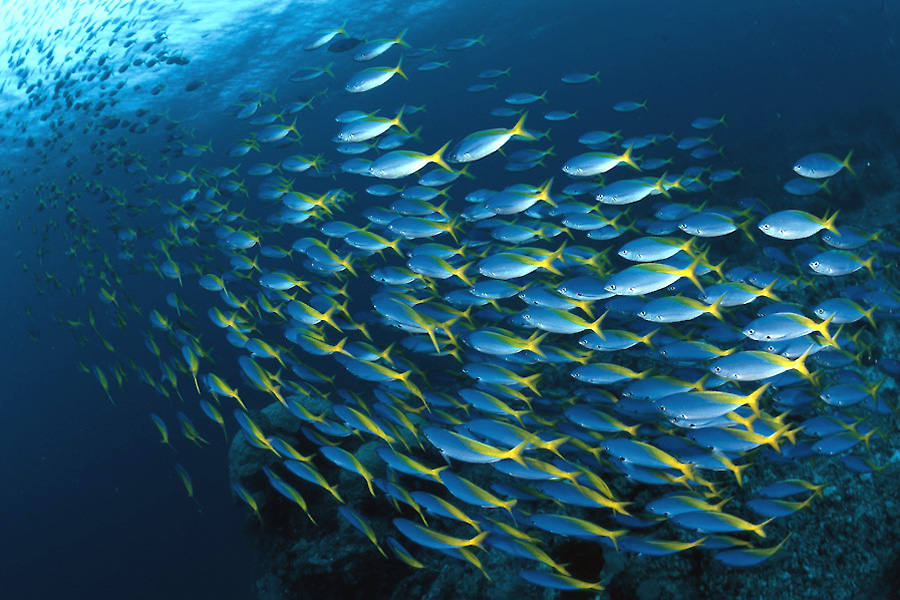
\includegraphics[width=0.4\textwidth]{images/technische_grundlagen/fischschwarm.jpg}
	\end{center}
	\caption{Fischschwarm}
	\label{fig:fischschwarm}
\end{wrapfigure}

\noindent
\paragraph{Ein Fischschwarm}
ist hierfür eines der bekanntesten Beispiele, indem die einzelnen Individuen des Schwarmes sich so verhalten, als würden sie wie ein einzelnes Tier agieren. Dabei setzt jeder Fisch feste Regeln um, die zur Umsetzung eines Schwarmverhaltens führen.
\begin{enumerate}
	\item Folge deinem Vordermann
	\item Behalte die Geschwindigkeit deines Nachbarn bei
\end{enumerate}
\noindent
Die wichtigste Rolle spielt hierbei der Schwellenwert zur Steuerung des Schwarms durch einzelne Teilnehmer. Da jedes Individuum den Schwarm durch seine Bewegung beeinflusst, existiert ein Schwellenwert, der sich einer Mindestanzahl von etwa fünf Prozent der Fische richtet, durch die der Schwarm gesteuert werden kann.\footnote{\citep[vgl.][Logistik Schwarmintelligenz]{Stober.Logistik:Schwarmintelligenz}\label{note47}} Somit reagieren die Fische ausschließlich auf die Mehrheit und der Schwarm lässt sich nicht durch eine Minderheit Fehlsteuern. Dieses Szenario lässt im Sinne von Veranstaltungen auf Menschen übertragen, um zu festzustellen an welchen Positionen Sicherheitspersonal positioniert werden muss, um einen geregelten Ablauf zu gewährleisten.\footref{note47}
\begin{wrapfigure}{r}{0.45\textwidth}
	\begin{center}
		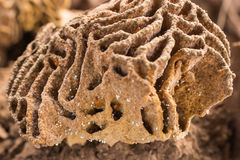
\includegraphics[width=0.4\textwidth]{images/technische_grundlagen/termitenschwarm.jpg}
	\end{center}
	\caption{Termitenschwarm}
	\label{fig:termitenschwarm}
\end{wrapfigure}

\noindent
\paragraph{Ein Termitenschwarm} geht nach dem Prinzip der Stigmergie vor, wie andere Insekten, die vorwiegend in einem Staat leben. Dabei kommunizieren die einzelnen Individuen indirekt über die Beeinflussung ihrer Umgebung, wie dem Hinterlassen von Spuren als Merkmale.\footnote{\citep[vgl.][Roboter bauen im Schwarm nach dem Vorbild von Termiten]{Schoenebeck.Roboterbauen}\label{note48}} Dieses Prinzip befähigt den kleinsten und primitivsten Organismen einen evolutionären Vorteil zu erlagen, indem sie sich nicht allein den Gefahren stellen, sondern in einer großen Masse zusammenarbeiten.\\
Dies ermöglicht ihnen das Bauen riesiger Nester, indem die Insekten einen ihren vorgegebenen inneren Plan, mit ihrer aktuellen Umgebung vergleichen und dadurch intuitiv erkennen, welche Arbeit sie zu erledigen haben.\footref{note48}\\

\noindent
Der Ablauf ist dabei folgender:
\begin{enumerate}
	\item Erkennen
	\item Analysieren
	\item Reagieren
\end{enumerate}
Dieses Prinzip lässt sich durch festlegen von Regeln auf Roboterschwärme abbilden, um wie Insekten vollkommen autonom Gebäude und andere Objekte durch den Einsatz einer indirekten Kommunikation zu errichten.

\subsubsection{Szenarien}

Zur Umsetzung verschiedener Schwarmverhalten lassen sich nützliche Teile der Tierwelt auf Roboter abstrahieren, um eine Zusammenarbeit der einzelnen Individuen effizienter zu gestalten. Hierbei werden meist mehrere Basisszenarien eingesetzt, die einerseits die Kommunikation, oder die Abläufe verbessern.\\
Für die Umsetzung der Kommunikation der einzelnen Teilnehmer existieren zwei verschiedene Möglichkeiten, einerseits eine direkt, oder indirekte Kommunikation. Dabei kann bei einer direkten Kommunikation auf die bekannten Kommunikationsmittel zurückgegriffen und über ein existierendes Netzwerk kommuniziert werden. Dabei wird meist nach dem bekannten Request-Response-Prinzip vorgegangen.
\begin{enumerate}
	\item Anfrage
	\item Verarbeitung
	\item Antwort
\end{enumerate}
Bei einer indirekte Kommunikation analysiert der Roboter dagegen seine Umgebung, um daraus Veränderungen zu registrieren und entsprechend zu reagieren. Dabei wird bei einer Umsetzung zur Implementierung folgend vorgegangen:
\begin{enumerate}
	\item Datenerfassung durch Sensorik
	\item Datenauswertung
	\item Vergleich der Datensätze
	\item Reaktion und Ausführung
\end{enumerate}
Für die Umsetzung eines Schwarmverhaltens, können viele Szenarien herangezogen werden, je nachdem, welche Problemstellung gelöst werden soll. Da sich dieses Projekt auf mobile Kleinroboter bezieht kommen folgende Basisszenarien in Frage:
\begin{itemize}
	\item Synchrone Verhaltensweise
	\item Verfolgung eines Objektes
	\item Selbstständige Verhaltensweise
\end{itemize}

\begin{wrapfigure}{r}{0.4\textwidth}
	\begin{center}
		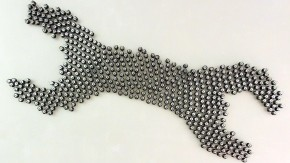
\includegraphics[width=0.35\textwidth]{images/technische_grundlagen/roboterform.jpg}
	\end{center}
	\caption{Roboter bilden Formen \cite{FrankfurterAllgemeineZeitungGmbH.Schwarmverhalten:Roboter}}
	\label{fig:roboterFormen}
\end{wrapfigure}

\paragraph{Die Synchrone Verhaltensweise} stellt einen Schwarm dar, wobei alle Individuen als Einheit agieren und somit ein großes Tier nachahmen. Dazu werden meist den jeweilig beteiligten Robotern dieselben Informationen zur Verfügung gestellt, um eine gleichmäßige Reaktion zu erreichen. Dies dient dazu spezielle Formen mit Robotern darzustellen und den gesamten Schwarm zu steuern.

\begin{verbatim}
\end{verbatim}
\newpage

\begin{wrapfigure}{r}{0.4\textwidth}
	\begin{center}
		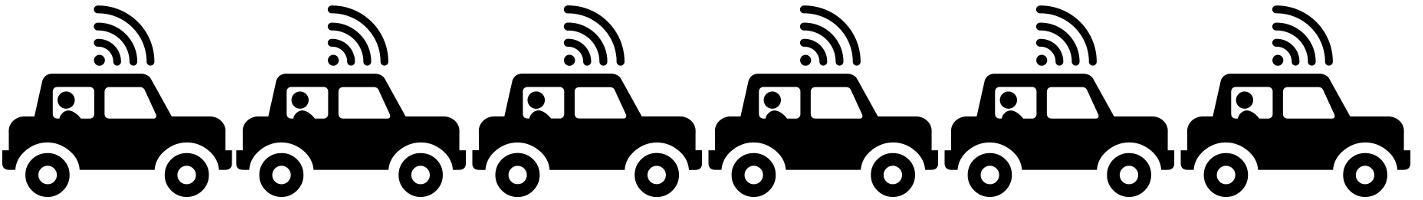
\includegraphics[width=0.35\textwidth]{images/technische_grundlagen/verkehr.png}
	\end{center}
	\caption{Roboter bilden Formen \cite{ETHZuerich.InduzierterVerkehr}}
	\label{fig:verkehr}
\end{wrapfigure}
\paragraph{Die Verfolgung eines Objektes} stellt Roboter dar, welche einem klar definierten Objekt folgen. Dies kann durch verschiedene Prinzipien veranlasst werden. Einerseits kann ein Objekt durch vorhandene Sensorik erfasst und damit verfolgt werden. Andererseits kann eine Verfolgung mittels Positionsdaten, wie \gls{gps} realisiert werden. Dieses Prinzip eines Schwarmverhaltens erfasst damit ein weites Spektrum an Anwendungsgebieten, wie eine automatisierte Verkehrsführung oder der Verfolgung durch Drohnen, welche die Möglichkeit besitzen durch Gesichtserkennung Personen und Objekte zu erkennen.

\begin{wrapfigure}{r}{0.25\textwidth}
	\begin{center}
		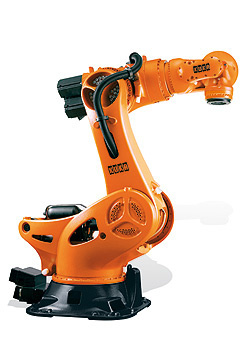
\includegraphics[width=0.2\textwidth]{images/technische_grundlagen/industrie.jpg}
	\end{center}
	\caption{Industrieroboter \cite{KUKA.IndustrieroboterKUKA}}
	\label{fig:industrie}
\end{wrapfigure}
\paragraph{Die Selbstständige Verhaltensweise} stellt eine indirekte Kommunikation zwischen Robotern dar, welche eine asynchrone Zusammenarbeit dieser ermöglicht. Dabei können unabhängig voneinander Roboter nach ihren Stärken für ein gemeinsames Ziel zusammenarbeiten. Dies findet oft Anwendung in Industrieanlagen, wobei jeder Roboter für eine spezielle Aufgabe ausgerüstet und programmiert ist. Diese erfassen zunächst das Produkt, um anschließend ihren definierten Arbeitsschritt durchzuführen.
